\documentclass[11pt, oneside]{book}
\usepackage[utf8]{inputenc}
\usepackage[english]{babel}
\usepackage{csquotes}
\usepackage{float}
\usepackage{booktabs}
\usepackage{caption}
\usepackage{subcaption}
\usepackage{amsmath}
\usepackage{amsfonts}
\newtheorem{theorem}{Theorem}[section]
\usepackage{multicol}
\usepackage{graphicx}
\usepackage{wrapfig}
\usepackage{tikz}
\usetikzlibrary{trees}
\usetikzlibrary{calc}
\usepackage{pgfplots}
\pgfplotsset{compat=1.18}
\usepackage{lineno}
\linenumbers
\usepackage[style=numeric-comp]{biblatex}
\addbibresource{bibliography.bib}
\usepackage{color, colortbl}
\definecolor{citegreen}{rgb}{0,0.5,0.2}
\usepackage{hyperref}
\hypersetup{
    colorlinks=true,
    linkcolor=blue,
    filecolor=magenta,
    urlcolor=cyan,
    citecolor=citegreen
}
\usepackage{listings}
\lstdefinestyle{mystyle}{
    keywordstyle=\color{purple},
    stringstyle=\color{green},
    basicstyle=\ttfamily\footnotesize,
    breaklines=true,                 
    captionpos=b,                    
    keepspaces=true,                 
    numbers=left,                    
    numbersep=5pt,                  
    showspaces=false,                
    showstringspaces=false,
    showtabs=false,                  
    tabsize=4
}
\lstset{style=mystyle}

\begin{document}

\pagenumbering{gobble}
\begin{center}
{\LARGE \textbf{University of Turin}}
\vspace{0.2cm}

{\Large {Computer Science Department}} 
\vspace{1cm}


\includegraphics[width=4cm]{figures/unito-logo.png}
\vspace{0.8cm}

{\Large {Master Thesis in Computer Science}}
\vspace{1cm}

{\LARGE \textbf{Quantum Approaches to \\Sentiment Analysis}}
\vspace{1cm}

\end{center}

\begin{multicols}{2}
\noindent \large{Supervisor:} \linebreak
\large{\textbf{Prof. Luca Roversi}} 
\vspace{0.1cm}

%\noindent {\large {Co-Supervisor:}} \linebreak
%\large{\textbf{???}} 
%\vspace{0.1cm}

%\noindent {\large {Controrelatore:}} \linebreak
%\large{\textbf{???}} 
%\vspace{0.1cm}
\columnbreak

\noindent{\large {Candidate:}} \linebreak
\large{\textbf{Mario Bifulco}} 
\end{multicols}
\vspace{2cm}

\begin{center}
    \large{\textbf{Academic Year 2023/2024}}
\end{center}



\newpage

\vfill
\section*{Statement of Originality}
I declare to be responsible for the content I am presenting to obtain the final degree, not to have plagiarised in all or part of the work produced by others and to have cited original sources in a way consistent with current plagiarism regulations and copyright. I am also aware that in the case of false declaration, I could incur in law penalties and my admission to the final exam could be denied.
\newpage

\section*{Acknowledgments}

Before presenting the work carried out during the months of this thesis, I would like to take a moment to thank the people without whom this endeavour would never have come to fruition.

First and foremost, I would like to express my gratitude to my supervisor, Luca Roversi. 
Throughout my academic journey, he has undoubtedly been the most influential figure, reigniting a passion that had begun to wane. 
His guidance in preparing this thesis allowed me to delve into topics of personal interest, granting me considerable autonomy while never leaving me feeling ``abandoned''. 
Thank you, not only for being an exceptional mentor but also for the profound humanity with which you support your students throughout their journey.

Despite my efforts, many of the results achieved would not have been possible with such ease if not for the unwavering support of my parents. 
Thanks to them, I could focus solely on my studies, taking the necessary time and making my mistakes. 
Not everyone has this opportunity, and I am deeply grateful for their constant presence. 
I cannot overlook my brother either—thank you for always bringing a smile to my face and for never knowing the answers to the math questions I ask you; you remind me that it's perfectly human not to have all the answers right away.

A special thanks to Silvia, who has patiently supported and stood by me since the beginning of university. 
You are perhaps the person who has most witnessed my frustration when I struggled to reach my goals. 
You have been, and continue to be my calm haven, and I hope you always will be.

I would also like to extend my gratitude to the Montano and Rozzino families, who represent a ``second family'' I can always rely on, no matter what.

Thanks to all the friends who accompanied me along the way, both long-time and recent, each contributing uniquely to this important milestone in my life.

Lastly, but by no means least, I want to thank my grandparents—this thesis is dedicated to you.

\pagenumbering{arabic}
\newpage

\section*{Abstract}
We initially investigate the application of a hybrid classical quantum classifier (HCQC) for sentiment analysis, comparing its performance against the classical CPLEX classifier and the Transformer architecture. 
Our findings indicate that the HCQC underperforms relative to the Transformer in terms of classification accuracy, but it requires significantly less time to converge to a reasonably good approximate solution. 
This investigation also reveals a critical bottleneck in the HCQC, whose architecture is partially undisclosed by the D-Wave property. 
To address this limitation, we propose a novel algorithm based on the algebraic decomposition of QUBO models, which enhances the time the quantum processing unit can allocate to problem-solving tasks.

\newpage

\tableofcontents
\newpage

\section*{Note on the Use of Quantum Solvers}

All the experiments using a quantum component have been conducted on real machines (hybrid or purely quantum) provided by D-Wave.
D-Wave offers a limited amount of free machine time each month, specifically 20 minutes for hybrid solvers and one minute for purely quantum solvers.
Once this limit is exceeded, users must either wait for the monthly renewal or opt for the ``premium'' option by paying additional computation time.

Ideally, the difference between the solvers available for free and those available through the premium version should pertain only to cost and the time allocated.
However, although this assumption seems reasonable, it is not explicitly confirmed in D-Wave's documentation.
For this reason, some of the considerations discussed may not apply equally when using the paid solvers.

\chapter{Introduction}

In recent years the development of models dedicated to the understanding and processing of natural language has significantly increased. 
With the public release of ChatGPT\cite{chatgpt}, the use of large language models has become accessible to anyone, enabling their rapid diffusion.

OpenAI, the company behind the development of GPT models, has shown\cite{scaling} that the quality of the model stems inevitably from a few fundamental aspects:
\begin{itemize}
    \item The quantity and relative quality of the data;
    \item The size of the model;
    \item The training time also depends on the computational infrastructure available.
\end{itemize}

The relationship between the quality or the quantity of data and the model's expressiveness is intuitive, even without the need to fully understand the architectural mechanisms of language processing models. 
A larger amount of data allows for extracting more examples of coherent sentences, thereby increasing the likelihood of accurately predicting the next word in a plausible sentence.
Furthermore, the information learned from the dataset is ``stored'' in the model's parameters, meaning high-quality data enables the model to manipulate text more effectively.

On the other hand, understanding why a larger model empirically yields better responses remains an open problem, explored in a different research field called Explainable AI.

As larger models require more data, there is also a need for greater computational power to train these models while limiting training time.
The resource demand is so high that training a ``foundational'' model, i.e., a large-scale model trained on general data, is feasible only for large tech companies such as Facebook, Google, and Microsoft.

\paragraph{Goals} This thesis studies alternative models that can reduce the required computational resources.
By working with unconventional computational architectures, this work aims to determine whether and how they can accelerate the creation of new models, correlating the increased speed with differences in the model's expressiveness.

The computational architecture on which the research has been conducted is adiabatic quantum computing (AQC, Section \ref{sec:AQC}), specifically its implementation is quantum annealing as proposed by D-Wave.
There are two primary reasons for this choice. 
First, adiabatic quantum computing naturally solves problems formulated in QUBO (quadratic unconstrained binary optimization) form.
Second, many deep learning training algorithms aim to minimize a function based on specific parameters.

Instead of using Transformer models, typically employed for language processing tasks, this thesis focuses on using support vector machines (SVM), shifting from deep learning to machine learning. 
Using SVMs (Section \ref{sec:svm}) allows for reducing the model's size from hundreds of millions of learnable parameters to a few tens of thousands, making it feasible to train the model even on personal computers or low-power systems such as embedded devices.

Rather than comparing the models in language modelling, the chosen task for language processing is Sentiment Analysis, specifically its binary version (BSA, Section \ref{sec:bsa}).
This task aims to separate sentences conveying a ``positive'' sentiment from those expressing a ``negative'' sentiment.

Using a well-defined task such as BSA allows for objectively evaluating the created model.
This is a substantial difference compared to language modelling, for which there are no standard evaluation datasets, and where better performance on synthetic benchmarks often does not lead to noticeable improvements in real-world applications.

By comparing the quantum implementation of BSA with state-of-the-art classical solvers and Transformer models, Section \ref{sec:qsvm-res} examines:
\begin{itemize}
    \item Performance relative to the classification task;
    \item Model training time;
    \item Time required to classify new examples.
\end{itemize}

From the analyses conducted, it appears that the use of the quantum processing unit (QPU) by D-Wave’s hybrid solvers is minimal.
Since the functioning of hybrid solvers is hidden by D-Wave’s intellectual property, it is impossible to explain this behaviour properly.
As discussed in Chapter \ref{sec:qpu}, the limited use of the QPU could stem from the inability to directly handle large-scale problems, as detailed in Section \ref{sec:me}.
To avoid excessive use of quantum resources, which are currently limited and costly to maintain, D-Wave might deliberately design hybrid algorithms that reduce QPU utilization.

An open question remains whether such design choices are applied only to non-paying users, as an incentive to encourage premium accounts, or if they are uniformly applied to all users.
Assuming no distinction is made between paying and non-paying users, the development of alternative hybrid solvers may not only allow the use of open-source software but also provide greater control over the amount of computation delegated to the QPU.

This topic is explored in more detail in the chapter \ref{sec:hsolver}, where an alternative solver to D-Wave is proposed, analysing the rationale behind its development and the performance achieved.

The alternative proposed in this thesis involves exploiting the algebraic properties of the QUBO problem in order to recursively partition large problems until they can be solved directly using QPU. The main purpose of this approach is to maximise the use of the QPU during the search for the global optimum.


\chapter{Theoretical framework}

This chapter will cover the main theoretical topics addressed during the development of the thesis. 
The aim of this exposition is not to exhaustively cover the research conducted in the various fields 
but to provide a sufficient overview to undertake the experimentation carried out.

\section{Sentiment Analysis}\label{sec:bsa}

The task of Sentiment Analysis\cite{SentAnalysis} finds its theoretical framework in the broader context of Natural Language Processing (NLP). 
NLP refers to algorithmic techniques aimed at manipulating, extracting information from, or generally ``understanding'' written text.

This field of research has roots in the early days of computer science and has always held significant interest for researchers in artificial intelligence.

Currently, the majority of natural language processing techniques employ deep learning models, 
particularly models based on the attention mechanism known as Transformers\cite{Attention}.

Sentiment Analysis is no exception, and the most promising models today are based on BERT\cite{BERT}, 
a method for encoding textual information that uses a contextual vector representation. 
This approach allows for the dynamic analysis of words, making it easier to capture the differences in meaning due to their position in the text.

Specifically, the task of Sentiment Analysis aims to classify provided examples into two or more classes based on the sentiment conveyed in the sentence. 
The binary version of this classification mechanism involves dividing the input data based on whether they transmit a ``positive'' or ``negative'' emotion.

The success of this type of classification is crucial in contexts such as social networks\cite{SentTweeter}, 
where these tools can enhance the ability of algorithms to autonomously moderate published content, 
thus avoiding excessive use of hate speech. 
Another application context where Sentiment Analysis is fundamental for optimal success is machine translation. 
Some languages are naturally more prone to the use of irony, 
and if this nuance of meaning is not captured, a ``naive'' translation would result in a completely meaningless output.

\section{Support vector machine}\label{sec:svm}

Among the various machine learning models for binary classification, support vector machines\cite{SVM} (SVMs) aim to separate examples by generalizing them as effectively as possible. The underlying idea is to select, among the candidate separation lines, the one that maximizes the distance between the elements of the two classes. Provided the training dataset is balanced, this procedure ensures better generalization properties for examples near the decision boundary that discriminates between positive and negative examples.

\begin{wrapfigure}{l}{0.45\textwidth}
    \centering
    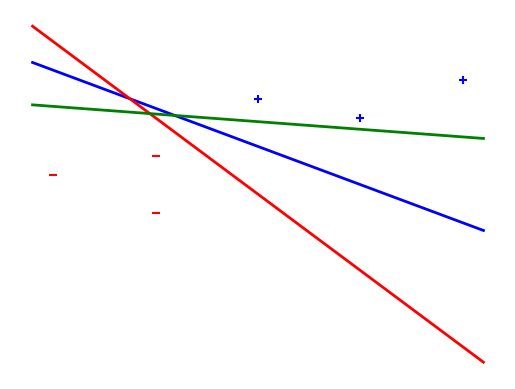
\includegraphics[width=0.4\textwidth]{figures/svm-intuition}
    \caption{Decision boundary.}
    \label{fig:svm-example}
\end{wrapfigure}

In Figure \ref{fig:svm-example}, we can visualize an example with two-dimensional data for classification. Among the different separation lines, it is intuitive to associate the blue one with the best generalization. This line not only correctly classifies all examples in the dataset but is also likely to generalize better during inference.

The formulation of SVMs is defined through a constraint satisfaction problem (CSP). To properly define the problem, it is necessary to introduce the notions of functional margin and geometric margin.

\paragraph{Functional Margin} The SVM model is described by a separating hyperplane represented by $f(x) = w \cdot x - t$. The functional margin is defined as $\mu(x) = y(w \cdot x - t) = yf(x)$. This function takes positive values if and only if the example is correctly classified. In the proposed formulation, $w$ and $t$ represent the model parameters to be derived during the learning phase. Intuitively, the functional margin indicates the rotation of the separation line in the example plane.

\paragraph{Geometric Margin} The geometric margin indicates the distance between the closest positive example to the decision boundary and the closest negative example. The formula to calculate its value is $\mu_g=(x_+-x_-)\cdot\frac{w}{||w||}$.

\begin{figure}[H]
    \centering
    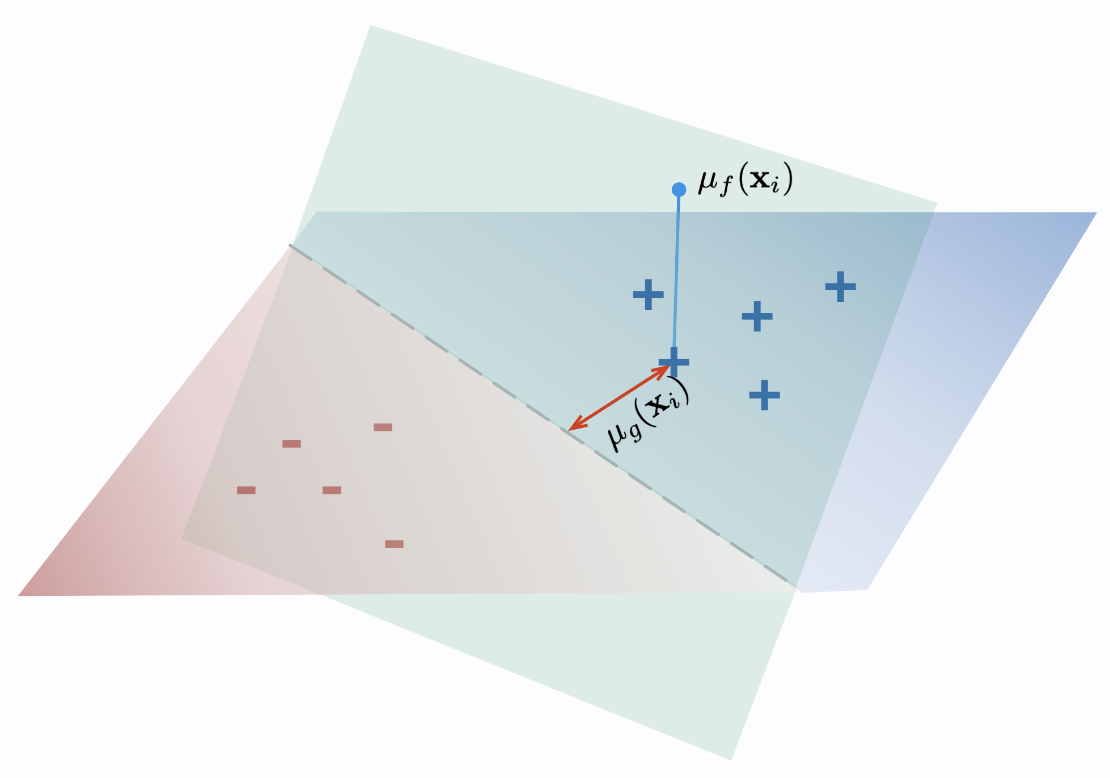
\includegraphics[width=0.7\textwidth]{figures/margins}
    \caption{Visual representation of the contribution of margins in defining the decision boundary.}
    \label{fig:svm-margins}
\end{figure}

\subsection{Primal Formulation}

The primal formulation of the optimization problem describing support vector machines takes the form:

\begin{align*}
    \min_{w, t}\ & \frac{1}{2}||w||^2 \\
    \text{subject to } & y_i(w \cdot x_i - 1)\geq 1 \quad \forall i:1\leq i\leq n
\end{align*}

In this case, the geometric margin is expressed in the objective function, while the functional margin is represented as a constraint of the problem.

\subsection{Derivation of the Dual Form}

The natural formulation for the problem, i.e., the primal, is not sufficiently efficient in terms of computation. However, its dual reformulation possesses some desirable properties. For instance, the dual problem depends only on the support vectors, i.e., the training dataset examples that lie on the margin.

The dual formulation for SVMs is derived starting from the Lagrangian relaxation.

$$\Lambda(w, t, \alpha) = \frac{1}{2}||w||^2 - \sum_{i=1}^n\alpha_i(y_i(w\cdot x_i - t) - 1)$$

This can be expanded into:

$$\frac{1}{2}w\cdot w - w\cdot\sum_{i=1}^n\alpha_iy_ix_i + t\sum_{i=1}^n\alpha_iy_i + \sum_{i=1}^n\alpha_i$$

To find the Lagrangian dual, we need to calculate the minimum of this function, which requires finding when the partial derivatives concerning $w$ and $t$ are zero.

$$\frac{\partial\Lambda}{\partial t} = \sum_{i=1}^n\alpha_iy_i = 0$$

$$\frac{\partial\Lambda}{\partial w} = w - \sum_{i=1}^n\alpha_iy_ix_i = 0 \to w = \sum_{i=1}^n\alpha_iy_ix_i$$

Substituting the results from the derivatives into the problem yields the dual formulation.

\begin{align*}
    \max_\alpha\ & -\frac{1}{2}\sum_{i=1}^n\sum_{j=1}^n\alpha_i\alpha_jy_iy_jx_ix_j + \sum_{i=1}^n
  \alpha_i \\
    \text{subject to } & 0 \leq \alpha_i \quad \forall i: 1\leq i\leq n \\
    & \sum_{i=1}^ny_i\alpha_i=0
\end{align*}

\subsubsection{Soft Margin}\label{sec:soft}

The previously discussed problem does not allow for any error from the model, meaning that, in the case of non-linearly separable data, it will be impossible to find an optimal assignment for the CSP. This behavior is undesirable. To address this, the problem can be relaxed to accept the presence of errors.

Thus, the constraint of the functional margin in the primal problem is modified to $y_i(w\cdot x_i-t)\geq1-\xi_i$, while the objective function is augmented with the component $C\sum_{i=1}^n\xi_i$, where $C$ is a predefined parameter that indicates the penalty weight introduced by the errors.

Deriving the problem yields:

\begin{align*}
    \max_\alpha\ & -\frac{1}{2}\sum_{i=1}^n\sum_{j=1}^n\alpha_i\alpha_jy_iy_jx_ix_j + \sum_{i=1}^n
  \alpha_i \\
    \text{subject to } & 0 \leq \alpha_i \leq C \quad \forall i: 1\leq i\leq n \\
    & \sum_{i=1}^ny_i\alpha_i=0
\end{align*}

\subsubsection{Kernel Trick}

The introduction of the soft margin is not sufficient to handle most real-world problems. Simple datasets can be constructed where it is impossible to find a linear separation that does not produce a high error rate during inference.

A mapping function is introduced to project the dataset points into a higher-dimensional space.

\begin{theorem}[Cover]
  A pattern classification problem cast in a nonlinear high-dimensional space is more likely to be linearly separable than in a low-dimensional space\cite{ThCover}.
\end{theorem}

Instead of performing the multiplication $x_ix_j$, this multiplication can be substituted with $\langle\phi(x_i), \phi(x_j)\rangle$. For efficiency reasons, these inner product can be precomputed by generating the kernel matrix $K(x_i, x_j) = \langle\phi(x_i),\phi(x_j)\rangle$. Using kernel matrices allows the calculation of the result value without explicitly computing the mapping of each element. This difference, which might seem secondary at first glance, is fundamental as it allows the use of kernels that map to a potentially infinite-dimensional hyperspace.

Kernels can thus be used in the dual formulation of SVMs to generalize classification to datasets with non-linearly separable data.

\begin{align}
    \label{eq:svm-obj}
    \max_\alpha\ & -\frac{1}{2}\sum_{i=1}^n\sum_{j=1}^n\alpha_i\alpha_jy_iy_jK(x_i, x_j) + \sum_{i=1}^n\alpha_i \\ 
    \label{eq:svm-c1}
    \text{subject to } & 0 \leq \alpha_i \leq C \quad \forall i: 1\leq i\leq n \\
    \label{eq:svm-c2}
    & \sum_{i=1}^ny_i\alpha_i=0
\end{align}

\subsubsection{Inference with the Dual Solution}

Solving the problem using the dual formulation does not directly provide the values of $w$ and $t$. These values need to be derived to use the result in the inference phase.

The coefficient $t$ can be calculated as an average of the results obtained with the support vectors.

$$t = \frac{\sum_{i=1}^n y_i - \sum_{j=1}^n(\alpha_jy_jK(x_i,x_j))}{n}$$

As for the value of $w$, it cannot be directly derived when using the kernel function. The new $f(x)$ formulation becomes:

\begin{equation}
  f(x)=\sum_{i=1}^n\alpha_iy_iK(x_i, x) + t\label{eq:svm-predict}
\end{equation}

\section{Adiabatic quantum computing}

To overcome some of the limitations of classical computing, alternative architectures have been developed. Prominent among these is quantum computing, a branch of information theory that has achieved important milestones in recent years, enabling its application in real-world contexts.

The two paradigms currently in use when discussing quantum computing are the gate-based approach and the adiabatic approach.

\subsection{Gate-based quantum computing}

Gate-based quantum computing involves the direct manipulation of qubits using quantum gates\cite{QGate}. This low-level approach is analogous to working directly with logic gates in a classical architecture. Quantum gates (distinct from classical gates) enable the creation of true general-purpose computational models, capable of performing any type of calculation. The computational advantage arises from the use of quantum phenomena, such as entanglement, and the use of superposition to ``search'' for the solution to a problem by exploring multiple states simultaneously, collapsing the solution only at the moment of measurement.

IBM is a leading company in this field, currently operating quantum computers with a qubit count in the hundreds.

\begin{figure}[H]
  \centering
  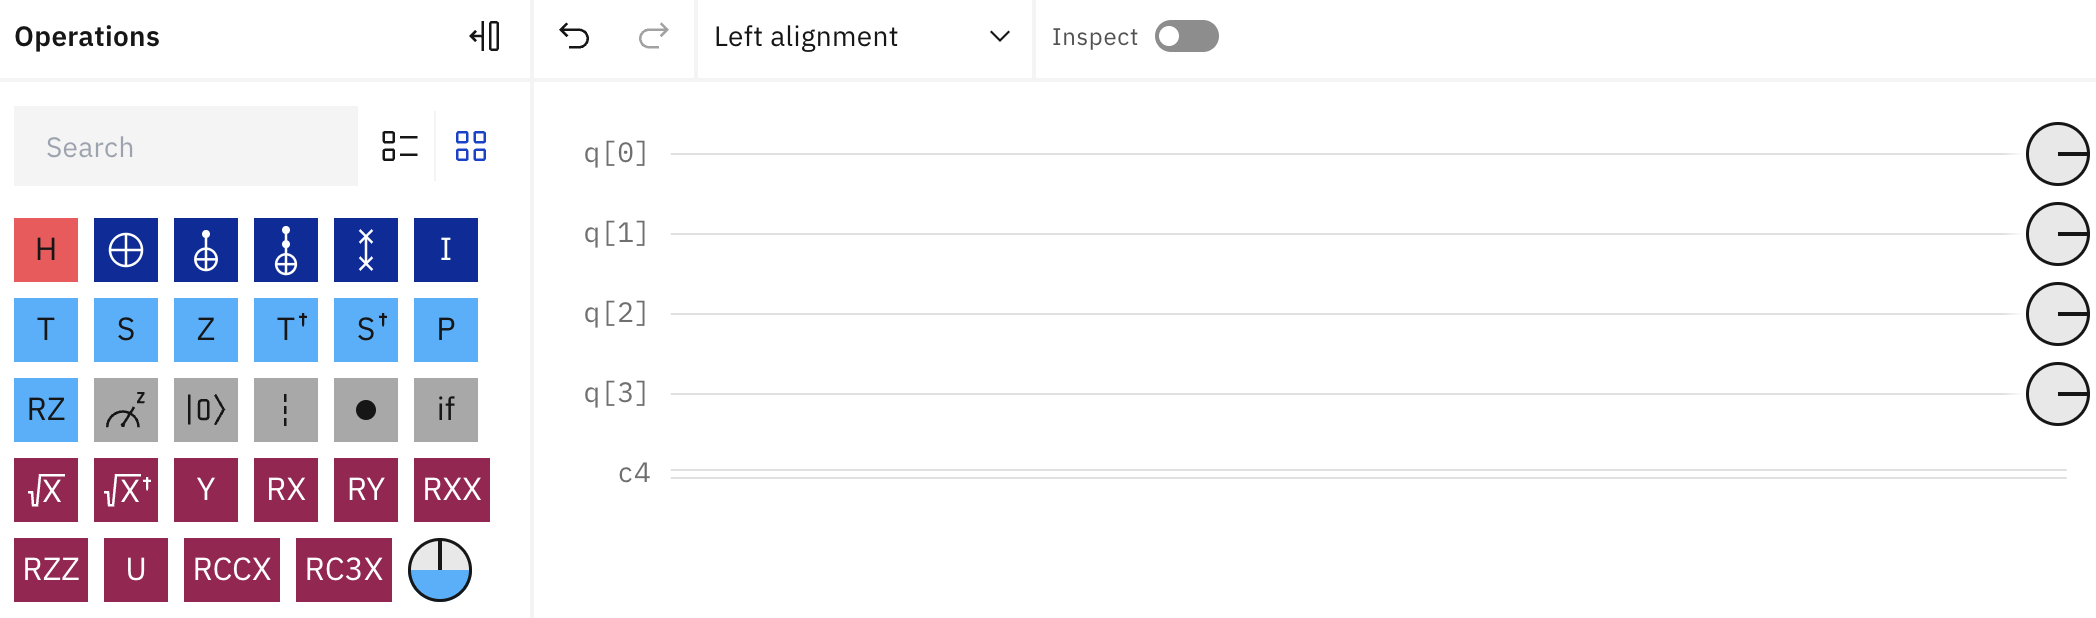
\includegraphics[width=\textwidth]{figures/4qubit}
  \caption{IBM quantum composer. Available gates and qubit system.}
\end{figure}

Although gate-based architecture represents a more generic computational model, the limitations due to the number of qubits and the error rates of these systems have led to the development of alternatives that can be used with the resources available. The most promising among these is adiabatic quantum computing.

\subsection{Adiabatic-based quantum computing}\label{sec:AQC}

Adiabatic quantum computing\cite{AQC} (AQC) is not aimed at creating a complete computational system. Instead, its goal is to exploit quantum phenomena to accelerate the optimization of models\cite{AQC2}. Specifically, D-Wave’s implementation of AQC follows these logical steps:

\begin{enumerate}
  \item Transform the problem into a Quadratic Unconstrained Binary Optimization (QUBO) formulation.
  \item Convert the objective function into a minimization problem.
  \item Generate the graph that represents the problem.
  \item Map this graph onto the qubit graph that forms the Quantum Processing Unit (QPU).
  \item Use quantum annealing to return the assignment that minimizes the objective function.
\end{enumerate}

This overview is a high-level representation of the steps required to utilize quantum annealing technologies. The complexity of the procedure is not immediately apparent at this level of abstraction, necessitating a detailed analysis of each step for a comprehensive understanding.

\paragraph{Minimization of Problems in QUBO Form} QUBO, an acronym for Quadratic Unconstrained Binary Optimization, is a standard formulation for expressing satisfaction problems. Specifically, all the information is encapsulated in the objective function, which takes the form $x^T Q x$, where $x$ is a column vector representing the optimization variables (with binary domain) and $Q$ is an upper triangular matrix describing the relationships between the variables. 

\begin{center} 
  $\underbrace{\begin{bmatrix}
      x_1 & \cdots & x_n 
  \end{bmatrix}}_{\bar{x}^T}$ 
  $\underbrace{\begin{bmatrix}
      a_1 & \cdots & a_n \\
      \vdots & \ddots & b_n \\
      0 & \cdots & c_n 
  \end{bmatrix}}_{Q}$ 
  $\underbrace{\begin{bmatrix}
      x_1 \\
      \vdots \\
      x_n 
  \end{bmatrix}}_{\bar{x}}$       
\end{center}

For use with adiabatic quantum computing, the QUBO problem must be in minimization form. Without loss of generality, any maximization problem can be transformed into a minimization problem, yielding the standard form for quantum machines: $\min x^T Q x$.

\paragraph{Problem graph for QUBO} The QPU does not directly manipulate QUBO problems but searches for the state with the lowest entropy (or energy) of a graph. The QUBO representation can be naturally rewritten into an undirected graph. The coefficients in the matrix $Q[i, j]$ represent the weight of the edge from node $i$ to node $j$. In the case of coefficients on the main diagonal, the edges enter and exit the same node.

For example, consider the following QUBO problem:

\begin{center} 
  $\begin{bmatrix}
    x_1 & x_2 & x_3 & x_4
  \end{bmatrix}$
  $\begin{bmatrix}
    -3 & 5 & 1 & -7 \\
    0 & 1 & 0 & 8 \\
    0 & 0 & 9 & -4 \\
    0 & 0 & 0 & -2 
  \end{bmatrix}$
  $\begin{bmatrix}
    x_1 \\ x_2 \\ x_3 \\ x_4
  \end{bmatrix}$      
\end{center}

Generates the following undirected graph:

\begin{figure}[H]
  \centering
  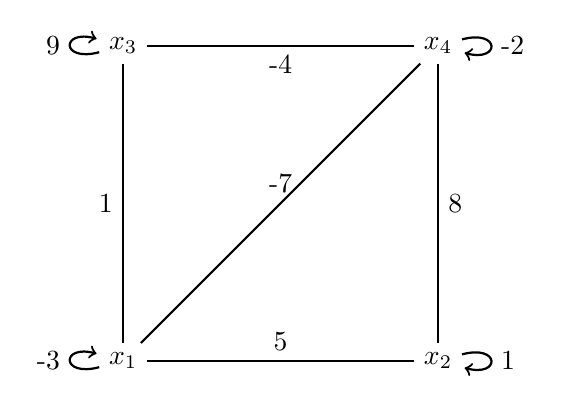
\begin{tikzpicture}
    \node (x1) at (0, 0) {$x_1$};
    \node (x2) at (4, 0) {$x_2$};
    \node (x3) at (0, 4) {$x_3$};
    \node (x4) at (4, 4) {$x_4$};

    \path[draw, thick] 
      (x1) edge[above] node{5} (x2)
      (x1) edge[left] node{1} (x3)
      (x1) edge[above] node{-7} (x4)
      (x2) edge[right] node{8} (x4)
      (x3) edge[below] node{-4} (x4);
  
    \path[draw, thick, looseness=10, out=135, in=225] 
      (x1) edge[loop left] node{-3} (x1)
      (x2) edge[loop right] node{1} (x2)
      (x3) edge[loop left] node{9} (x3)
      (x4) edge[loop right] node{-2} (x4);
  \end{tikzpicture}
  \caption{Graph of the proposed problem.}
  \label{fig:problem-graph}
\end{figure}

\paragraph{Minor graph embedding} As previously mentioned, the structure of the QPU\cite{Pegasus} is fixed, and this structure determines the number and connections between the Qubits.

Imagining a QPU with 32 Qubits, its shape would be approximately as follows:

\begin{figure}[H]
  \begin{center}
      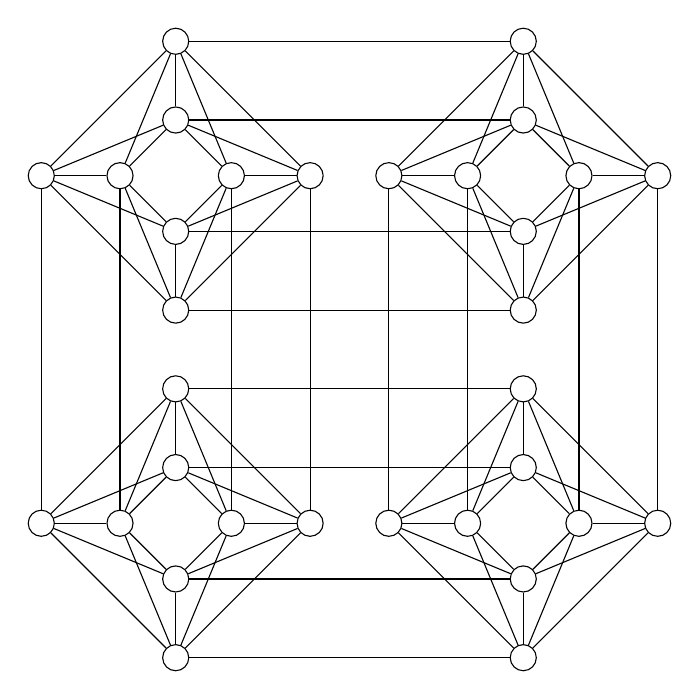
\begin{tikzpicture}[main/.style = {draw, circle}] 
          \node[main](1){};
          \node[main](2)[right of=1]{}; 
          \node[main](5)[above right of=2]{};
          \node[main](6)[above of=5]{};
          \node[main](3)[below right of=5]{};
          \node[main](4)[right of=3]{};
          \node[main](7)[below right of=2]{};
          \node[main](8)[below of=7]{};
  
          \draw (1) -- (6);\draw (6) -- (4);\draw (4) -- (8);\draw (8) -- (1);
          \draw (1) -- (5);\draw (5) -- (4);\draw (4) -- (7);\draw (7) -- (1);
          \draw (6) -- (2);\draw (2) -- (8);\draw (8) -- (3);\draw (3) -- (6);
          \draw (2) -- (5);\draw (5) -- (3);\draw (3) -- (7);\draw (7) -- (2);
          \draw (1) -- (2);\draw (5) -- (6);\draw (3) -- (4);\draw (8) -- (7);
  
          \node[main](11)[right of=4]{};
          \node[main](12)[right of=11]{}; 
          \node[main](15)[above right of=12]{};
          \node[main](16)[above of=15]{};
          \node[main](13)[below right of=15]{};
          \node[main](14)[right of=13]{};
          \node[main](17)[below right of=12]{};
          \node[main](18)[below of=17]{};
  
          \draw (11) -- (16);\draw (16) -- (14);\draw (14) -- (18);\draw (18) -- (11);
          \draw (11) -- (15);\draw (15) -- (14);\draw (14) -- (17);\draw (17) -- (11);
          \draw (16) -- (12);\draw (12) -- (18);\draw (18) -- (13);\draw (13) -- (16);
          \draw (12) -- (15);\draw (15) -- (13);\draw (13) -- (17);\draw (17) -- (12);
          \draw (11) -- (12);\draw (15) -- (16);\draw (13) -- (14);\draw (18) -- (17);
  
          \node[main](26)[below of=8]{};
          \node[main](25)[below of=26]{};
          \node[main](22)[below left of=25]{};
          \node[main](21)[left of=22]{};
          \node[main](23)[below right of=25]{};
          \node[main](24)[right of=23]{};
          \node[main](27)[below right of=22]{};
          \node[main](28)[below of=27]{};
  
          \draw (21) -- (26);\draw (26) -- (24);\draw (24) -- (28);\draw (28) -- (21);
          \draw (21) -- (25);\draw (25) -- (24);\draw (24) -- (27);\draw (27) -- (21);
          \draw (26) -- (22);\draw (22) -- (28);\draw (28) -- (23);\draw (23) -- (26);
          \draw (22) -- (25);\draw (25) -- (23);\draw (23) -- (27);\draw (27) -- (22);
          \draw (21) -- (22);\draw (25) -- (26);\draw (23) -- (24);\draw (28) -- (27);
  
          \node[main](36)[below of=18]{};
          \node[main](35)[below of=36]{};
          \node[main](32)[below left of=35]{};
          \node[main](31)[left of=32]{};
          \node[main](33)[below right of=35]{};
          \node[main](34)[right of=33]{};
          \node[main](37)[below right of=32]{};
          \node[main](38)[below of=37]{};
  
          \draw (31) -- (36);\draw (36) -- (34);\draw (34) -- (38);\draw (38) -- (31);
          \draw (31) -- (35);\draw (35) -- (34);\draw (34) -- (37);\draw (37) -- (31);
          \draw (36) -- (32);\draw (32) -- (38);\draw (38) -- (33);\draw (33) -- (36);
          \draw (32) -- (35);\draw (35) -- (33);\draw (33) -- (37);\draw (37) -- (32);
          \draw (31) -- (32);\draw (35) -- (36);\draw (33) -- (34);\draw (38) -- (37);
  
          \draw (6) -- (16);
          \draw (5) -- (15);
          \draw (7) -- (17);
          \draw (8) -- (18);
          \draw (26) -- (36);
          \draw (25) -- (35);
          \draw (27) -- (37);
          \draw (28) -- (38);
          \draw (1) -- (21);
          \draw (2) -- (22);
          \draw (3) -- (23);
          \draw (4) -- (24);
          \draw (11) -- (31);
          \draw (12) -- (32);
          \draw (13) -- (33);
          \draw (14) -- (34);
      \end{tikzpicture} 
      \caption{32 QuBit QPU.}
      \label{fig:QPU}
  \end{center}
\end{figure}

The structure of the Qubits is characterized by this ``diamond'' shape that D-Wave calls Pegasus. The currently available QPUs have approximately 5500 Qubits, in which a pattern similar to the one shown in figure \ref{fig:QPU} is repeated.

To embed the graph \ref{fig:problem-graph} into the QPU, the nodes must be arranged appropriately. Direct mapping is not always possible, and in such cases, the minor embedding procedure\cite{ME} is necessary. The minor embedding algorithm constructs chains of qubits that map multiple physical nodes of the QPU to the same logical node of the original graph. This approach compensates for the limited connections of the QPU and ensures all necessary nodes are connected.

A possible embedding for \ref{fig:problem-graph} might be:

\begin{figure}[H]
  \begin{center}
      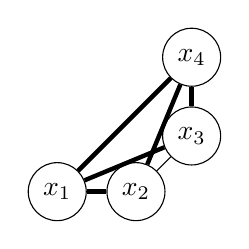
\begin{tikzpicture}[main/.style = {draw, circle}] 
          \node[main](1){$x_1$};
          \node[main](2)[right of=1]{$x_2$}; 
          \node[main](5)[above right of=2]{$x_3$};
          \node[main](6)[above of=5]{$x_4$};
  
          \draw[ultra thick] (1) -- (6); \draw[ultra thick] (1) -- (5); \draw[ultra thick] (6) -- (2); 
          \draw[ultra thick] (5) -- (6); \draw[ultra thick] (1) -- (2); \draw (2) -- (5);
      \end{tikzpicture} 
      \caption{Embedded problem}
      \label{fig:embedding}
  \end{center}
\end{figure}

\paragraph{Quantum annealing} 

Once the graph is mapped onto the QPU, the search for the assignment that minimizes the energy expressed by the physical system can begin. The two main phenomena during this process are annealing and quantum tunnelling.

The annealing phenomenon (referred to as thermal jump in figure \ref{fig:q-anneal}), which is also present in various local search techniques like simulated annealing\cite{SimulatedAnnealing}, aims to escape local minima. The idea behind this technique is to allow a state change that temporarily increases the total energy, with the hope that from this new state, a global minimum can be reached.

To further avoid local minima, quantum computing leverages the tunnelling phenomenon. The physical system can naturally change states towards a more stable configuration with lower energy. This physical process helps avoid searching by climbing peaks, thus accelerating convergence towards the global minimum.

\begin{figure}[H]
  \centering
  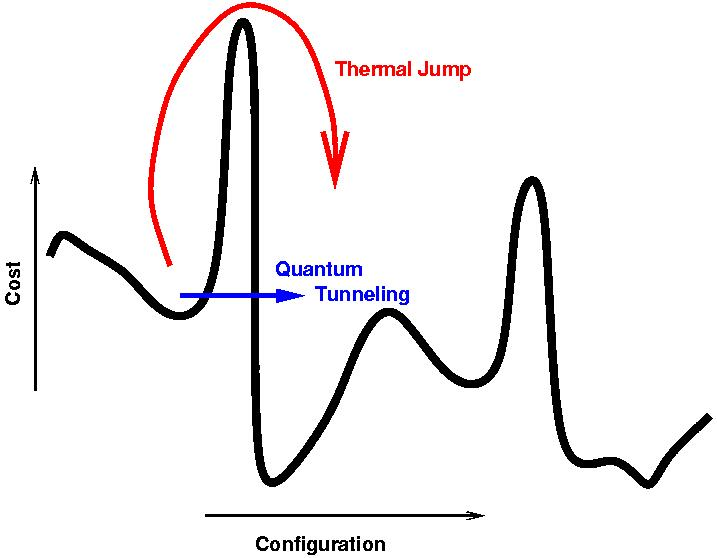
\includegraphics[width=0.5\textwidth]{figures/q-annealing.jpg}
  \caption{Graphical representation of quantum annealing.}
  \label{fig:q-anneal}
\end{figure}

\part{Quantum SVM for Sentiment Analysis}

\chapter{Motivations for the experimental setup}

The thesis project began with the intention of assessing the suitability, or unsuitability, of the quantum computing paradigm applied to a plausible case study within the realm of machine learning.

Among the various possibilities, sentiment analysis was chosen as the task. This decision was made because, in its traditional form, this task reduces to a binary classification. Being a preliminary step towards a potentially broader analysis that could combine natural language processing with quantum computing, it was reasonable to start with standard tasks that are well-documented and easy to verify in terms of results.

\section{Advantages of using non-deep learning}

Despite the dominance of deep learning models in the current landscape of computational linguistics research, using non-deep learning models provides greater flexibility for analysis. The hope in using ``simpler'' models is to understand their behaviour better, thus enabling the identification and correction of gross errors to improve performance during inference.

Among the various binary classification models, SVMs are the most promising choice. Other studies have shown that SVMs are the best machine learning model for text-related tasks\cite{ML4NLP}. Furthermore, their natural formulation makes them extremely versatile regarding input data, allowing the use of the most appropriate textual embedding for the chosen context. Additionally, the equivalence between margin optimization in SVMs and certain aspects of the attention mechanism in Transformers can be demonstrated\cite{TransformerSVM}.

Finally, the formulation of SVMs as a constraint satisfaction problem (CSP) allows for potential comparisons with various computational techniques, including:

\begin{itemize}
    \item Gradient descent,
	\item Optimization on classical architecture,
	\item Optimization on quantum architecture,
\end{itemize}
in addition to comparisons with the benchmark, i.e.,  state-of-the-art deep learning models.

\section{Advantages of a quantum architecture}

Nearly all artificial intelligence models can be expressed as a minimization problem, particularly in the most commonly used architectures where the goal is to minimize the loss function to reduce the error on the training dataset. Although these processes cannot always be naturally rewritten as CSPs, we can imagine that some parts of the optimization process can be handled based on the objective functions and constraints of the problem.

SVMs lend themselves to a quantum reformulation as they are natively formulated as a constraint satisfaction problem with quadratic components\cite{QSVM}. Analyzing equations \ref{svm-obj}, \ref{svm-c1}, and \ref{svm-c2}, it can be seen that the optimization variables $\alpha$ appear as a quadratic component in the first part of the objective function and as a linear contribution in constraint \ref{svm-c2} and the second part of the objective function. Constraint \ref{svm-c1} can be temporarily ignored as it represents a restriction on the domain of $\alpha$.

Although quantum machines can solve many optimisation problems, it is reasonable to expect better performance in intrinsically quadratic problems. Linear optimisation problems, while expressible, may not have enough intrinsic complexity to justify an architectural change.

Having established why using SVMs on quantum machines could yield significant results, it is appropriate to hypothesize what to expect, to adequately contextualize the results that will be collected.

Quantum solvers promise to tackle optimization problems more efficiently and in less time. Unfortunately, it is not possible to evaluate the impact in terms of energy efficiency of this computing procedure. The power consumption of quantum chips should be negligible\cite{QPUefficiency}, but being part of an opaque system provided by D-Wave, it is not possible to record significant information. For this reason, the subsequent analysis will focus primarily on the time required to solve the optimization problem, seeking to understand if and when using a non-classical architecture can speed up the optimization processes.

\chapter{Problem posing}

\section{Manual conversion to QUBO form}

To utilize the quantum computing systems provided by D-Wave, the formulation of SVMs must be slightly modified. These minor adjustments are necessary to transform a CSP into a QUBO form.

First of all, it is essential to transform the objective function into a minimization problem due to the physical nature of how quantum machines seek solutions. To transform the current objective function, it is sufficient to invert the signs of each component in the sum because the optimal solution for $\max f(x)$ is equivalent to the best solution for $\min -f(x)$, resulting in:

\begin{equation}\label{eq:min-svm}
    \min_\alpha\ \frac{1}{2}\sum_{i=1}^n\sum_{j=1}^n\alpha_i\alpha_jy_iy_jK(x_i, x_j) - \sum_{i=1}^n\alpha_i
\end{equation}

Constraint \eqref{eq:svm-c2} can be incorporated into the objective function as a penalty constraint through Lagrangian relaxation. This procedure simplifies the finding of potential solutions since the problem’s constraints no longer need to be explicitly satisfied. However, by appropriately calibrating the Lagrangian multiplier, it is possible to ensure that the optimal solutions are those that satisfy the constraints, effectively reducing the penalty constraints to zero.

$$\min_\alpha\ \frac{1}{2}\sum_{i=1}^n\sum_{j=1}^n\alpha_i\alpha_jy_iy_jK(x_i, x_j) - \sum_{i=1}^n\alpha_i + L\left(\sum_{i=1}^ny_i\alpha_i\right)^2$$

An empirical method advises setting the Lagrangian parameter $L$ to a value between 70\% and 150\% of a bound of the solution calculated greedily\cite{QbridgeI}.

The final step to achieve a QUBO formulation is to rewrite the problem using binary variables. The presented SVM formulation uses the real domain for the variables $\alpha$, making them not directly usable. A ``naive'' solution to this problem could be to use a standard encoding for real numbers, similar to traditional computers, such as IEEE 754\cite{IEEE}. However, since each binary variable corresponds to a node in the QPU graph, this approach would be highly inefficient, requiring a large number of qubits that would essentially be underutilized.

Alternatively, ad hoc representations can be evaluated to minimize the number of qubits to the bare essentials. Using the information from constraint \eqref{eq:svm-c1}, which limits the domain of the variables $\alpha$ to positive numbers less than $C$, can be helpful. Additionally, machine learning models often do not require the full numerical precision available in modern computers, making it reasonable to consider limiting the precision of the expressible real numbers to a fixed number of decimal places, further reducing the number of qubits needed for a single $\alpha$.

A final possible refinement could be to use a numerical representation system based on powers of ten instead of powers of two. For instance, the four-bit number $1011$ could represent $10.11$ ($10^1 + 10^{-1} + 10^{-2}$) instead of $2.75$ ($2^1 + 2^{-1} + 2^{-2}$), in this representation system, the number of bits is divided equally between the integer and fractional parts.

The choice of the Lagrangian hyperparameter and the bit system to represent the optimization variables depends on the specific problem and the data considered.

\section{Automatic D-Wave conversion}\label{sec:dwaveconversion}

The previously described procedure can be performed automatically by the libraries provided by D-Wave. The products available through cloud computing relieve the developer of the responsibility of handling problems by imagining the qubit grid and instead allow writing only the mathematical formulation of the CSP, delegating the solver to transform and optimize the problem using the QPU.

This process is not done by directly accessing the quantum solver but through what are defined as hybrid solvers\cite{hybrid}. Intuitively, a hybrid solver prepares the problem on the QPU and divides the work between the QPU and CPU to speed up the optimization process by offloading the CPU from the more complex procedures.

Hybrid solvers can read the standard format in which optimization problems are written, allowing easier substitution of classical solvers with quantum solvers. For example, any optimization model written with Pyomo\cite{pyomo}, a standard library in combinatorial optimization, can save models in text files that can later be read and loaded into D-Wave’s internal solver format.

\paragraph{Domain limitations}\label{sec:domain} Reading the file describing the problem and converting it to the internal representation is entirely transparent as long as two conditions are met:
\begin{enumerate}
    \item The problem must be written in minimization form,
    \item There must be no multiplications between real variables.
\end{enumerate}
Equation \eqref{eq:min-svm} shows that it is not a problem to meet the first requirement. However, it is different regarding the multiplication of optimization variables in the real domain. The SVM formulation involves quadratic interactions between variables in the real domain. To approximate the solution without requiring a complete problem rewrite, it is possible to convert all variables to the integer domain. In this way, using the information from constraint \eqref{eq:svm-c1}, $\lceil\log_2(C)\rceil$ qubits are sufficient for each variable $\alpha$.

Empirically, the proposed approximation results in negligible performance deterioration while significantly reducing the number of qubits required for each variable.

\subsection{Pre-solving}\label{sec:presolve}

The guidelines provided by D-Wave to make best use of its hybrid solvers suggest performing the pre-solution operation for constrained quadratic models (CQM). This procedure aims to statically analyse the problem and eliminate redundant operations or restructure the problem to make the best use of available information.

While it is not always possible to guarantee optimal behaviour, pre-solving generally brings significant advantages during model resolution. Various strategies have been proposed in the literature, and state-of-the-art classical solvers autonomously implement similar policies to make the search more efficient.

Among the various techniques available, D-Wave implements some low-computational-cost strategies, all derived from \cite{PRESOLVE}.

\paragraph{Removal of redundant constraints} The removal of constraints is based on the structural limits of the problem. For instance, during the creation of SVMs, the variables $\alpha$ are declared as integers in $[0, C]$. Hence, a constraint like $\alpha_0 \geq 0$ is irrelevant since the information is contained in the domain of $\alpha$.

\paragraph{Removal of low magnitude bias} This operation is performed on both constraints and the objective function. Each solver has a parameter indicating the maximum difference to tolerate to consider two floating-point numbers equal, often called ``feasibility tolerance''. Some biases significantly below the ``feasibility tolerance'' can be rounded to zero since it is verified that they will never have significant impacts on the rest of the problem.

\paragraph{Domain propagation} Based on the problem constraints, the domain of the variables is reduced. This procedure not only limits the solutions but also has a desirable impact on the number of qubits required to express the problem variables. By reducing the domain, fewer nodes of the Pegasus graph are sufficient.

\paragraph{Note on pre-solving efficiency} The pre-solving strategy proposed by D-Wave has proven to have minimal impact in terms of computational overhead. A brief exploratory investigation showed that the number of nodes in the transformed problem could grow to double the original graph size. This behaviour could motivate specific cases where, although applicable, it might be optimal not to apply pre-solving to avoid excessive growth in the problem size.

In the specific case addressed, the problem dimensions are well below the system’s limits\cite{hybrid2}. Therefore, it is possible to take advantage of the pre-solving strategy.


\chapter{Testing framework}

\section{Dataset used}\label{sec:dataset}

To compare the proposed implementation with other machine learning models, both deep and non-deep, a standard dataset that allows for reasonable comparisons is necessary. In the literature, several datasets specifically developed for Sentiment Analysis can be found. Among these, TweetEval\cite{tweeteval} will be analyzed in detail.

TweetEval, a dataset proposed by CardiffNLP\footnote{\url{https://cardiffnlp.github.io/project/tweeteval/}}, contains various contexts of text classification. Among these, the ``sentiment'' split categorizes sentences based on the fundamental emotion they convey, whether positive, negative, or neutral. The golden standard includes 60,000 labelled examples extracted and subsequently anonymized from \url{https://x.com/}, previously known as Twitter. The strings extracted from the social network are concise, ranging from 10 to 200 characters, with 73.7\% of the examples being between 90 and 150 characters in length. The examples are distributed among the classes in an imbalanced manner, with 45\% belonging to the neutral class, 40\% labelled as positive, and only 15\% conveying negative emotions. The underrepresentation of the negative class may be due to content verification mechanisms on Twitter, which are tools designed to discourage overly aggressive use of the platform leading to a scarcity of negative sentences. 

The imbalanced nature of the dataset can be desirable in some contexts; generally, it is crucial to be aware of it to evaluate potential rebalancing strategies. 

In the presented context, a balanced dataset is preferable, because otherwise, the optimization process of SVMs might favour a \emph{dummy classifier}, i.e., a classifier that always responds with the majority class, as it minimizes error for the given data.

\section{Pre-processing Strategy}

Before the dataset can be used to train the models, some pre-processing operations are necessary. These operations ensure higher quality input data to improve the performance of the resulting models.

\paragraph{Eliminating Superfluous Class} SVMs allow for the classification of data divided into two classes. This working hypothesis may be too restrictive in some application contexts. Referring to the ``sentiment'' split of TweetEval, it is reasonable to expect that most tweets do not convey a specific sentiment, thus the need for the neutral class. Alternatively, one might require not only identifying a positive or negative sentiment but also associating the text with a specific emotion (hate, joy, fear, \dots).

In the situations described above, multi-class classification is necessary. In the literature, methods for transforming a multi-class classification into a set of binary classifications are available\cite{multiclass}. This procedure requires training multiple models that learn to classify different subsets of the total information, combining their results to identify the target class uniquely. 

Since this thesis does not focus on developing a ``production-ready'' solution, it is possible to focus on training a single binary classifier and studying its advantages and disadvantages. 

The reasoning conducted will be generalizable to multi-class dataset usage.

Among the three classes available in TweetEval, the neutral class is opted to be eliminated for two reasons:
\begin{enumerate}
    \item It is the most difficult class to classify even for a human;
    \item Given the distribution of the data in the classes of the dataset, sentences belonging to the neutral class appear to be the most numerous, however, training in the presence of scarce data can create classification problems, which is why the two least represented classes, the positive and the negative, are chosen.
\end{enumerate}

\paragraph{Mapping Labels for SVMs} The standard formulation of Support Vector Machines (SVMs) assumes the association of the positive class with $+1$ and the negative class with $-1$. This allows for the computation of the value of Equation \eqref{eq:svm-predict} and the determination of the class membership of example $x$ using the sign function.

Since the data in TweetEval are labelled with $0$ for the negative class and $2$ for the positive class, it is necessary to map the labels to the domain $\{-1, 1\}$. Otherwise, multiplication by zero would cause problems during optimization, reducing the whole Equation \eqref{eq:svm-obj} to zero. Additionally, the sign function would not be usable during inference. The simplest way to achieve this domain change is by subtracting $1$ from the original labels.

\paragraph{Balancing the Dataset} As reported in Section \ref{sec:dataset}, the distribution of examples across classes is not fair. The balanced dataset is a desirable property in SVMs, so the number of examples extracted from the positive class equals the cardinality of the negative one. Despite the significant reduction in the number of examples, the dataset is large enough to guarantee more than 5,000 instances for each class considered. For this reason, it is possible to resize the dataset without worrying about potential information loss.

\section{Generating Sentence Embeddings}\label{sec:embeddingused}

Current artificial intelligence models are not capable of ``understanding'' text, at least not in the intuitive sense associated with the verb understand, so it is needed to reprocess the information and transform a sequence of characters into a sequence of numbers. This process is known as \emph{embedding generation}.

Before deep-learning models, embeddings were manually built by identifying salient information from the text. For example, trying to separate ``simple'' words from ``complex'' ones. Some relevant information could be:
\begin{itemize}
    \item The part of speech represented, also known as PoS (noun, verb, adverb, \dots);
    \item The length of the word;
    \item The frequency in a reference dataset.
\end{itemize}

Deep neural networks have allowed the automatic creation of text embeddings with high semantic significance\cite{word2vec}. The newly generated vectors have significantly increased the number of dimensions, from tens to hundreds. The increase has considerably improved performance at the cost of making the embeddings uninterpretable; each word is mapped into a multidimensional space, but the semantic meaning of a single axis is unknown.

To further improve performance, ad hoc variants of embeddings for specific tasks\cite{sentimentEmbedding} or procedures to capture the information of an entire sentence\cite{sentence-bert} have been developed.

In the analysed application context, generating an embedding for the entire sentence can be considered an appropriate choice. 
\begin{itemize}
    \item On the one hand, it avoids shifting the complexity of the Sentiment Analysis task from the model to the embedding, as would happen using ad hoc embeddings for the reference task.
    \item On the other hand, it allows a sufficiently expressive vector representation to be produced.
\end{itemize}

The embeddings for TweetEval were generated using the pre-trained \verb|all-mpnet-base-v2| model, which transforms a sentence into a vector in 768 dimensions. The input sentence used to create the embedding must be shorter than 384 characters; since the reference dataset works on short sentences, this constraint is not limiting.

\section{Processed Dataset}\label{sec:tweetdf}

Upon completion of the pre-processing operations, the dataset derived from TweetEval will henceforth be referred to as TweetDF. The data contained in TweetDF are divided into two main subsets.

The train set contains 14,000 examples, of which 7,000 belong to the positive class, labelled $1$, and 7,000 belong to the negative class, labelled $-1$.

The test set contains 4,000 new examples, equally distributed between the positive and negative classes.

Each entry in TweetDF contains:
\begin{itemize}
    \item The text in natural language;
    \item The sentence embedding, a 768-dimensional vector;
    \item The associated label, which is the target of the classification.
\end{itemize}


\chapter{Results}

\section{Classification Methodologies Compared}\label{sec:qsvm-res}

The analysis focuses on comparing three fundamental aspects that characterize each machine learning model:
\begin{enumerate}
    \item The quality of the classification;
    \item The time required for the training phase;
    \item And the time needed to classify new examples.
\end{enumerate}

In the subsequent analyses, times will be reported in seconds. Since both training and inference are considered waiting times: 
\begin{itemize}
    \item The former for obtaining the actual model;
    \item The latter for obtaining the relevant data.
\end{itemize}

The best result will be closest to zero, i.e., the procedure that takes the least time to provide the desired result.

Evaluating performance is not as straightforward because a wrong choice of judgment method may highlight secondary flaws and conceal potential strengths. Conversely, it could lead to the opposite situation, concluding that the proposed approach is better than it should be.

As this is a binary classification task, classic machine-learning metrics can be utilized. The data obtained from the inference phase are divided based on the original labels of the dataset, assigning the \emph{Actual Positive} (AP) set to the data labelled $1$ and the \emph{Actual Negative} (AN) set to the data labelled $-1$. Test data are also divided based on the class produced by the model, generating the \emph{Predicted Positive} (PP) and \emph{Predicted Negative} (PN) sets. Based on these four sets, the \emph{contingency table}, Table \ref{tab:contingency}, is determined.

\begin{table}[h]
    \centering
    \begin{tabular}{l|ll}
       & PP & PN \\\hline
    AP & TP & FN \\
    AN & FP & TN
    \end{tabular}
    \caption{Contingency table}
    \label{tab:contingency}
\end{table}

The intersection between two of the above-described sets defines:
\begin{itemize}
    \item \emph{True Positive} (TP), the elements of the positive class categorised correctly;
    \item \emph{False Positive} (FP), elements of the negative class that were classified as positive;
    \item \emph{True Negative} (TN), elements correctly classified as negative;
    \item \emph{False Negative} (FN), elements erroneously labelled as negative.
\end{itemize}

From the values in the contingency table, various evaluation metrics can be derived, all of which are within the interval $[0, 1]$, where $0$ indicates the worst possible value and $1$ is the perfect score.

\paragraph{Accuracy} $\frac{TP + TN}{TP + TN + FP + FN}$, indicates the number of correct predictions out of the total available examples, thus not providing explanations for the errors obtained.

\paragraph{Precision} Derived using the formula $\frac{TP}{TP + FP}$, it indicates how many of the elements labelled as positive should have been positive.

\paragraph{Recall} From the formula $\frac{TP}{TP + FN}$, it provides a measure of how well a relevant datum (positive class) is correctly interpreted by the model.

\paragraph{F1-Score} The formula is obtained through the harmonic mean of precision and recall, $2*\frac{\text{Precision}*\text{Recall}}{\text{Precision}+\text{Recall}}$. This metric avoids degenerate situations where a desirable result is obtained on one of the two metrics while significantly decreasing the score of the other.

These four metrics will be considered for evaluating the obtained models, to capture as much information as possible for assessing performance during the classification of new examples.

\section{Performance Analysis}

Using the APIs provided by D-Wave, it is possible to calculate the minimum time required by a CSP problem, Section \ref{sec:qadvantages}, to be solved by the hybrid solver available.

To tackle the optimisation problem generated by TweetDF, section \ref{sec:tweetdf}, the expected calculation time is approximately 480 seconds, due to the number of optimisation variables $alpha$ in \ref{eq:min-svm}, each one associated with an example of the training set. 
This calculation time is excessively high compared to the free version of D-Wave's hybrid resolution services, which are limited to 20 minutes.

To conduct a larger number of iterations and extract the average behaviour, the size of the dataset can be reduced, allowing for faster resolution. 
An appropriate compromise between the number of examples and the time required by the hybrid solver was obtained using a dataset of 4096 examples for the model training phase. 
These examples were randomly selected from TweetDF, ensuring an equal number of elements of the positive and negative classes. 
In contrast, the number of examples for the inference phase was reduced to 2048 elements.

The subset extraction of the data was performed randomly, only imposing an equal number of positive and negative examples.

The results obtained from ten distinct executions are reported in Tables \ref{tab:QSVM1}, \ref{tab:QSVM2}, and \ref{tab:QSVM3}. These tables are presented to allow a comparison with classical methods for solving the same classification task, represented by CPLEX and RoBERTa.

\paragraph{Classical Optimizer CPLEX} The CPLEX program\cite{cplex} is an optimization software for solving linear and non-linear programming problems. The mathematical formulation of the CSP describing an SVM is represented using the PyOmo library, which allows abstraction concerning the chosen solver and the generic writing of problems. Once the problem is formulated as an objective function and constraints, calls to the optimization library are made, returning the assignment of the variables $\alpha$ that minimizes the objective function \ref{eq:min-svm}. The results regarding the resolution of the problem through CPLEX are detailed in Table \ref{tab:QSVM1}.

\begin{table}[h]
    \centering
    \begin{tabular}{ccccccc}
    \toprule                                                             \\                    
    Train time & Accuracy & Precision & Recall & F1    & Time to predict \\
    \midrule
    285.207    & 0.8      & 0.95      & 0.64   & 0.77  & 2.324           \\
    278.999    & 0.83     & 0.91      & 0.74   & 0.81  & 1.997           \\
    267.266    & 0.81     & 0.97      & 0.65   & 0.77  & 2.059           \\
    256.59     & 0.8      & 0.96      & 0.64   & 0.76  & 2.353           \\
    254.312    & 0.78     & 0.95      & 0.59   & 0.73  & 2.105           \\
    271.298    & 0.81     & 0.93      & 0.68   & 0.79  & 2.383           \\
    271.301    & 0.79     & 0.91      & 0.64   & 0.75  & 2.392           \\
    266.922    & 0.82     & 0.93      & 0.69   & 0.79  & 2.148           \\
    257.671    & 0.79     & 0.96      & 0.61   & 0.75  & 2.398           \\
    264.427    & 0.8      & 0.88      & 0.68   & 0.77  & 1.977           \\
    \bottomrule
    \end{tabular}
    \caption{Results obtained through CPLEX}
    \label{tab:QSVM1}
\end{table}

\paragraph{Hybrid Optimizer from D-Wave} D-Wave offers a suite of hybrid solvers, for optimization problems, available through Python APIs\cite{hss}. The program is always initialized using the PyOmo library and then transferred to D-Wave's cloud services for resolution. Unlike CPLEX, which returns a single optimal solution, the solver provided by D-Wave produces a list of possible assignments, each with its associated objective function value. By extracting all and only the assignments with the minimum objective function value, it is possible to produce a set of models and perform the inference phase by aggregating the individual results through a majority vote. Although this procedure slows down the prediction, it could improve the inference phase. The results obtained using the solvers proposed by D-Wave are detailed in Table \ref{tab:QSVM2}.

\begin{table}[h]
    \centering
    \begin{tabular}{ccccccccc}
    \toprule
    Train time & Accuracy & Precision & Recall & F1    & Time to predict \\
    \midrule
    390.745    & 0.81     & 0.97      & 0.64   & 0.77  & 40.219          \\
    423.917    & 0.79     & 0.96      & 0.6    & 0.74  & 30.186          \\
    326.422    & 0.79     & 0.97      & 0.59   & 0.73  & 23.686          \\
    239.25     & 0.76     & 0.95      & 0.55   & 0.7   & 19.74           \\
    221.635    & 0.81     & 0.96      & 0.65   & 0.77  & 39.708          \\
    320.892    & 0.8      & 0.96      & 0.63   & 0.76  & 34.159          \\
    319.161    & 0.81     & 0.96      & 0.65   & 0.78  & 40.224          \\
    437.813    & 0.82     & 0.97      & 0.67   & 0.79  & 40.424          \\
    377.309    & 0.81     & 0.97      & 0.65   & 0.78  & 30.541          \\
    220.48     & 0.82     & 0.97      & 0.66   & 0.79  & 39.654          \\
    \bottomrule
    \end{tabular}
    \caption{Results obtained through D-Wave}
    \label{tab:QSVM2}
\end{table}

\paragraph{The Transformer Model RoBERTa} In addition to the optimization methods reported, it is relevant to evaluate the performance of the D-Wave hybrid solvers compared to the state-of-the-art. The model considered belongs to the BERT family. The foundational version of RoBERTa\cite{roberta-base} was trained on the Sentiment Analysis task using datasets of various natures, taking approximately 15 days to converge. Subsequently, the model was fine-tuned on TweetEval\cite{tweetRoberta}\cite{robertamodel} to specialize it in classifying ``basic'' sentiments.

\begin{table}[h]
    \centering
    \begin{tabular}{ccccc}
    \toprule
    Accuracy & Precision & Recall & F1    & Time to predict \\
    \midrule
    0.95     & 0.95      & 0.94   & 0.95  & 142.569         \\
    0.94     & 0.94      & 0.94   & 0.94  & 124.094         \\
    0.94     & 0.94      & 0.93   & 0.94  & 141.828         \\
    0.95     & 0.95      & 0.94   & 0.95  & 133.949         \\
    0.94     & 0.95      & 0.93   & 0.94  & 147.302         \\
    0.94     & 0.95      & 0.93   & 0.94  & 135.804         \\
    0.94     & 0.95      & 0.93   & 0.94  & 136.883         \\
    0.94     & 0.95      & 0.93   & 0.94  & 132.836         \\
    0.95     & 0.96      & 0.94   & 0.95  & 137.382         \\
    0.94     & 0.95      & 0.94   & 0.94  & 135.044         \\
    \bottomrule
    \end{tabular}
    \caption{Results obtained through RoBERTa}
    \label{tab:QSVM3}
\end{table}

Considering the results reported in different contexts, the following analysis is done of the three characteristics of interest identified in the Section \ref{sec:qsvm-res}.

\paragraph{Performance during Inference} The results recorded by RoBERTa are significantly better compared to those obtained from SVMs, both in the quantum version and the CPLEX classical one.
The first score recorded by CPLEX, Table \ref{tab:QSVM1}, shows 0.77 as F1, the same score is obtained by the hybrid D-Wave solver, Table \ref{tab:QSVM2}, while on the same dataset RoBERTa obtains an F1 score of 0.95, thus increasing by more than 20\%.

Despite this, the machine learning models also report scores well above a random guess, leading to the conclusion that the proposed methodology can capture the semantic information conveyed by the text, although not as well as the Transformer architecture, which is renowned in the literature for its superior ability to convey textual information. No significant differences are noted between the model produced by D-Wave and the one generated with CPLEX, indicating that the reduction in the optimization variable domain, discussed in \ref{sec:domain}, does not impact model performance.

\paragraph{Training Time} Although unavailable, the training times for an expressive and fine-tuned model like RoBERTa are certainly higher than those recorded by the optimization approaches. 
At the very least, it is reasonable to expect times in the order of hours, if not days, on high-performance GPUs. 
Conversely, the D-Wave approach and the one based on CPLEX allowed training the model on a personal computer. 
The recorded times, between 250 and 450 seconds, consider several external factors such as:
\begin{itemize}
    \item The need to convert the data into a suitable format to be processed by the optimisation procedure, which takes about 80 seconds;
    \item For D-Wave optimizer, sending the model to the cloud infrastructure, while it is not possible to record the time taken to transmit the data, one can consider the size of the CSP on disk, which is around 4GB.  
\end{itemize} 
Analyzing only the time required to produce the response to the problem, the CPLEX optimizer takes an average of 100 seconds, while D-Wave's hybrid computation produces comparable quality responses in only 40 seconds, significantly reducing the required time.

\paragraph{Classification Time} When inferring new examples, the times recorded by RoBERTa were the worst of the three methodologies compared. 
Although in this case, the unit of measurement is still seconds, the time required to classify the same number of new examples is significantly greater. 
Among the SVM variants, classical and quantum, the version produced by D-Wave is less performant than that obtained with CPLEX. 
This behaviour is due to the use of multiple models to calculate the result, a procedure not performed with the result obtained from CPLEX. 

\subparagraph{Improving D-Wave Classification Time} From a qualitative analysis of the ensemble procedure, using multiple models does not seem to bring particular benefits; In almost all cases, the majority class equals the class predicted by each model in the set. 
For this reason, it is possible to avoid the computational overhead of the ensemble procedure and use only one of the optimal models obtained through D-Wave, which reduces inference time, making the results produced by CPLEX and D-Wave comparable.

\section{Testing with the whole dataset}

Since the results obtained from different executions are almost identical, it is possible to perform a single test using the entire TweetDF. This additional test allows verification of the consistency of performance across the entire data set and the scalability of the hybrid optimisation.

\begin{table}[h]
    \centering
    \begin{tabular}{cccccc}
    \toprule
    \multicolumn{6}{c}{D-Wave}                                       \\ \midrule
    Train (min) & Accuracy & Precision & Recall & F1   & Predict (s) \\
    35          & 0.82     & 0.96      & 0.66   & 0.78 & 212.3       \\ \bottomrule
    \toprule
    \multicolumn{6}{c}{RoBERTa}                                      \\ \midrule
                & Accuracy & Precision & Recall & F1   & Predict (s) \\
                & 0.94     & 0.95      & 0.94   & 0.94 & 291         \\ \bottomrule
    \end{tabular}
    \caption{Results with whole TweetDF}
    \label{tab:qsvm-fulldf}
\end{table}

The results shown in Table \ref{tab:qsvm-fulldf} pertain to RoBERTa and D-Wave. The data regarding CPLEX are not reported since the SVM problem with such a large dataset caused the optimizer to crash before producing a result. This incident highlights a significant advantage of quantum computing: the ability to handle not only more complex problems but also larger ones. This is relevant because, in general, the more information encoded in the problem, the better the optimal solution produced.

\paragraph{Performance during Inference} The performance results do not vary significantly, indicating that a random subset of TweetDF is sufficient to capture the semantic information that can be modelled with SVMs.

\paragraph{Training Time} The training time using D-Wave rises to 35 minutes, of which 8 minutes are used on the D-Wave hybrid solver. 
Despite the considerable increase in training times, the optimization conducted by D-Wave is still much shorter than what is reasonable to expect for training RoBERTa.

\paragraph{Classification Time} The simultaneous use of several models by D-Wave has a significant impact on the time required to infer the class of new examples. While RoBERTa's inference times are even longer, the difference is insufficient to justify an architectural change. By using only one of the equivalent models presented by D-Wave's hybrid solver, it would be possible to reduce the calculation time and generate answers more efficiently.

\section{QSVM Overview}

In summary, machine-learning approaches conducted with CPLEX and D-Wave showed:
\begin{itemize}
    \item To converge quickly to the optimal solution, requiring a small dataset size and not taking advantage of the increase in input data;
    \item To approximate Transformer performance within an acceptable range in contexts where time and computational power constraints are involved, such as embedded systems and personal computers.
\end{itemize}

Specifically, the approach leveraging quantum computing (D-Wave) has proven to be superior to classical optimization (CPLEX), allowing for solving the presented problems in less time and with comparable performance.


\part{Maximizing quantum boost}

\chapter{Using the QPU Directly}\label{sec:qpuonly}

\section{Analysis of Hybrid Solving Times}

Section \ref{sec:qsvm-res} has shown that adiabatic quantum computing can offer advantages in terms of faster convergence to a solution. However, it is worth asking how much of this advantage is due to the quantum component and how much is attributable to a classical solver optimised for quadratic problems.

The technology behind the hybrid solvers is protected by D-Wave's intellectual property, which makes these tools essentially black boxes. 

Given the proprietary nature of these solvers, analysis must rely on the limited data available to make informed evaluations of alternative solutions.
From the control dashboard provided by D-Wave\footnote{\url{https://cloud.dwavesys.com/leap/}}, it is possible to inspect the problems solved by their QPUs and obtain some useful information.

Although the data collected does not allow an in-depth analysis of the underlying implementation choices, it can still be useful for a ``high-level'' analysis.
\begin{figure}
    \centering
    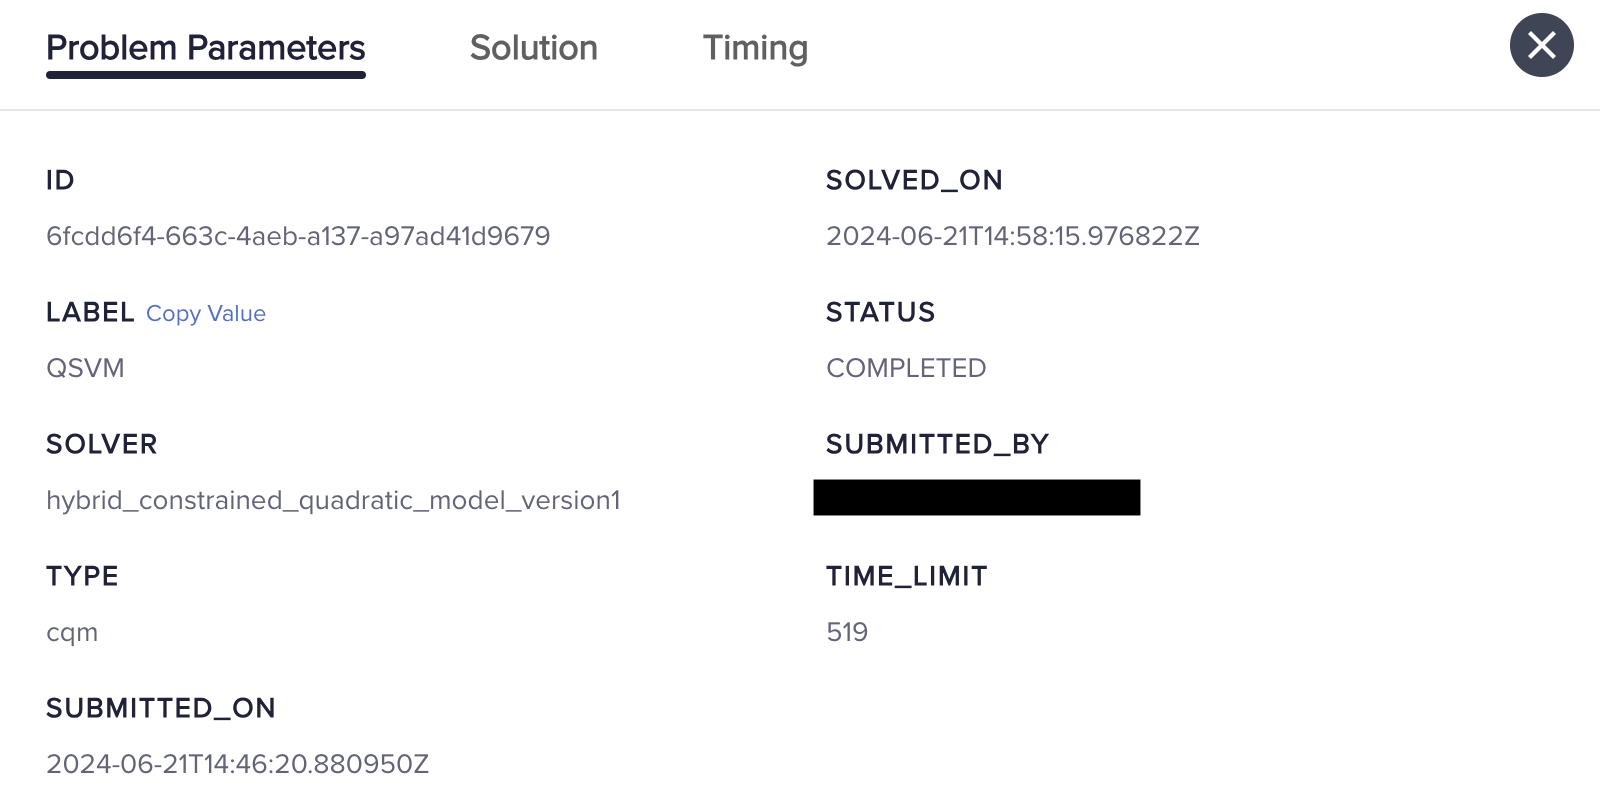
\includegraphics[width=0.8\textwidth]{figures/dashboard.png}
    \caption{D-Wave Leap dashboard.}
    \label{fig:dwaveleap}
\end{figure}
By selecting a problem from the list, the information from Figure \ref{fig:dwaveleap} is available, i.e: 
\begin{itemize} 
	\item A report on the characteristics of the problem presented, whether BQM, QUBO or CQM. 
	\item A list of the calculated potential solutions, together with the associated energy values, representing the result of the objective function with the given assignment. Figure \ref{fig:sampleset} is an example. 
	\item Execution times of the problem, indicating not only the total time but also how much of this time was spent on the QPU. Namely ``Timing'' tab of Figure \ref{fig:dwaveleap}
\end{itemize}

\begin{figure}
    \centering
    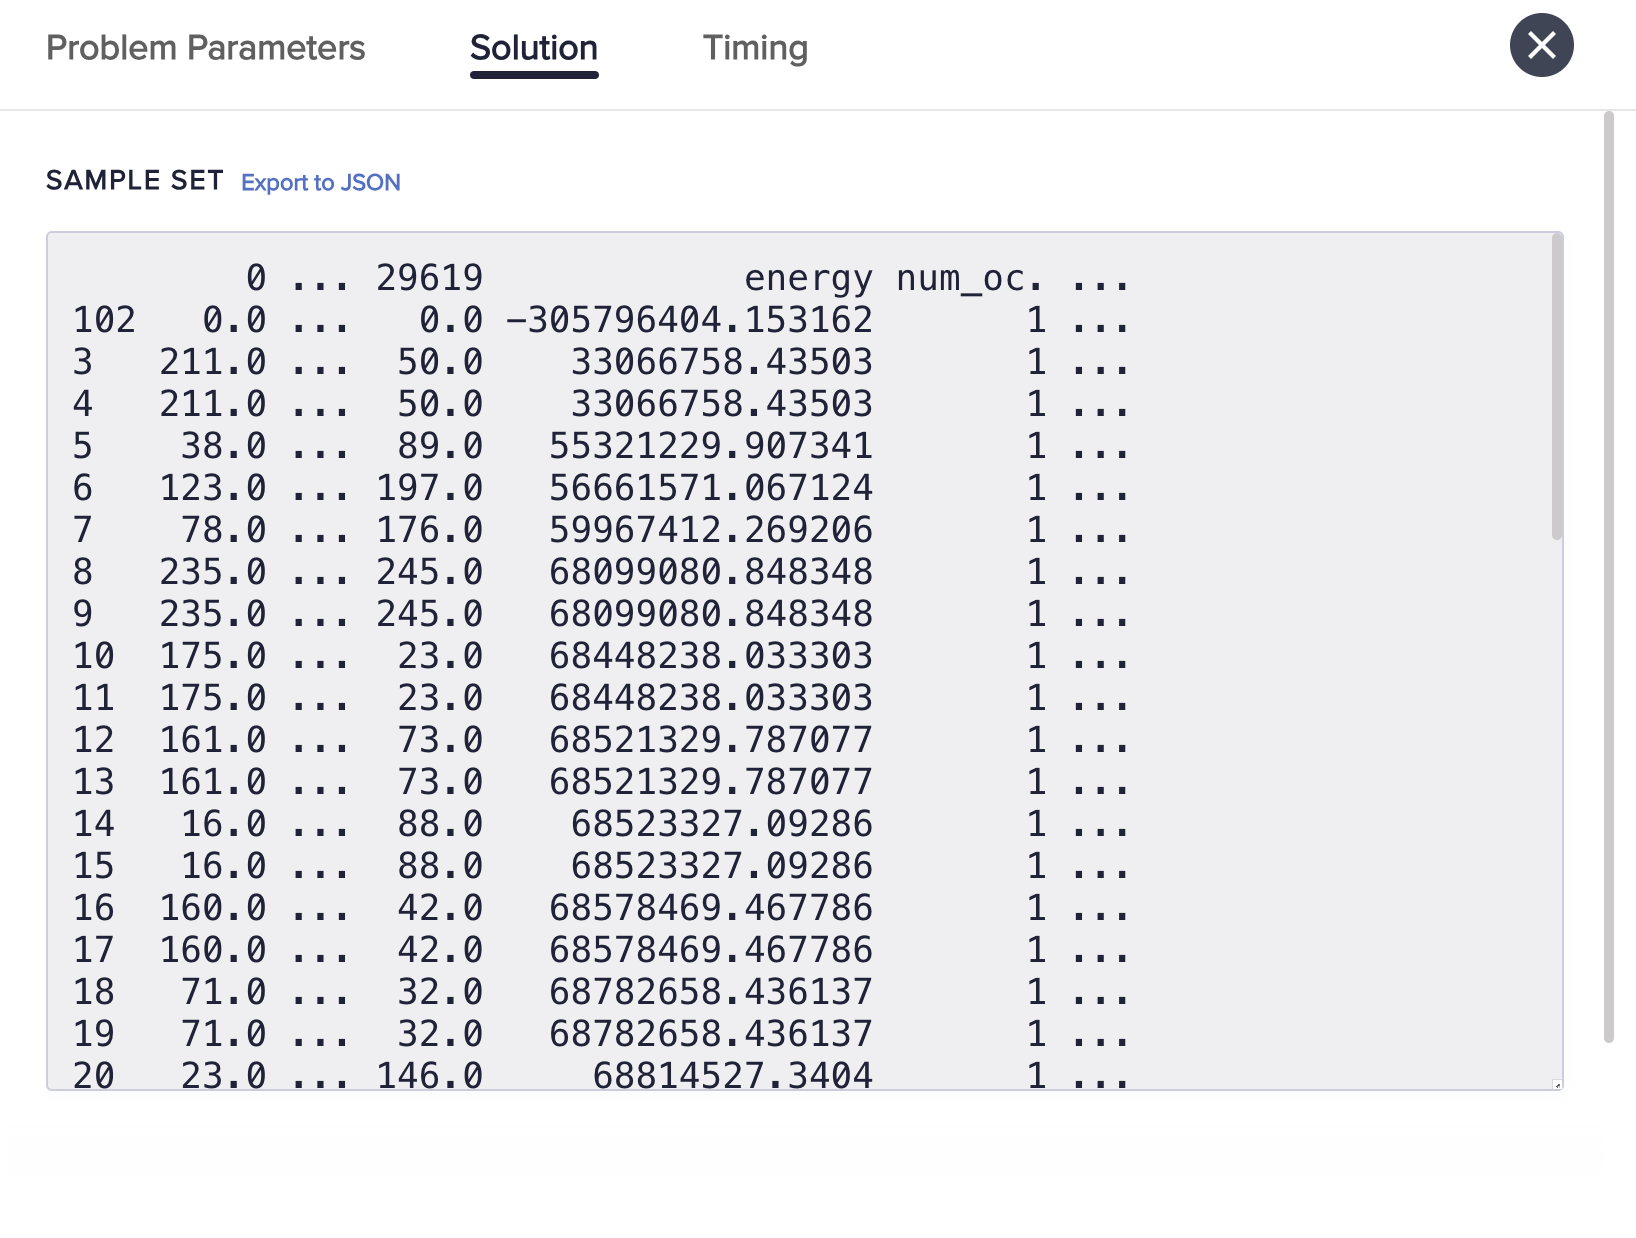
\includegraphics[width=0.8\textwidth]{figures/sampleset.png}
    \caption{List of solutions.}
    \label{fig:sampleset}
\end{figure}

Of the available data, information on execution time is of main interest, as it can help to determine whether and to what extent the quantum component is crucial in generating an optimal solution.

\subsection{QPU Usage}\label{sec:qpuusage}

Analysing the execution of the quantum support vector machine on a subset of TweetDF, it can be seen that of the 40 seconds it took to find the optimal solution, only 0.031 seconds were used by the QPU. Proportionally, the QPU was used for only 0.08\% of the total time required by the solver.

When using the entire TweetDF, the data indicated a QPU utilisation of 0.05 seconds, compared to the 480 seconds it took the solver to find a solution, reducing the QPU utilisation to 0.01\%.

These results highlight two fundamental aspects: 
\begin{itemize} 
	\item The use of the QPU is minimal compared to the classical component required to calculate the solution; 
	\item The use of the QPU seems to decrease as the problem size increases, while the time used by the classical component increases significantly. 
\end{itemize}

Considering that the D-Wave hybrid solver has proven to be more efficient than its classical counterpart, CPLEX, the question arises whether the performance improvement is due to the QPU or a superior classical solver.

As an alternative to D-Wave's hybrid approach, ``QPU-only'' solvers can be used. By manually performing the pre-processing steps, the classical reprocessing and resolution component can be avoided, while the entire calculation is performed on the QPU.

\paragraph{Free use of quantum solver} It is important to note that all observations made in this study pertain to behaviours recorded using the free tier of D-Wave's solvers. 
This plan offers 20 minutes per month for the hybrid solvers and one minute per month for purely quantum solvers.

It is not explicitly stated whether the paid plan involves using different algorithms compared to the free version. 
Given that, some of the findings gathered may not fully reflect the complete potential of the quantum technology provided by D-Wave.

\section{QPU solver}

The use of purely quantum solvers provided by D-Wave necessitates two main steps before a problem can be submitted to the QPU:

\begin{enumerate}
    \item Conversion of the problem into QUBO form;
    \item Transformation into an equivalent problem compatible with the QPU.
\end{enumerate}

As discussed in Section \ref{sec:dwaveconversion}, the former can be performed automatically using the libraries provided by D-Wave, which convert a problem expressed as an objective function and constraints (CSP) into an equivalent QUBO problem, i.e., $x^TQx$, as outlined in Section \ref{sec:AQC}.

The latter is related to minor embedding, which involves transforming the problem into an equivalent form that respects the qubit structure of the QPU.

The operations necessary to convert a CSP into a QUBO form can be executed in linear time. Therefore, if it were possible to perform minor embedding without requiring excessive computational resources or time, the use of the QPU without leveraging the hybrid component would present itself as a valid methodology for solving problems through adiabatic quantum computing.

The following sections will thus focus on analyzing the minor embedding algorithm, examining what has been implemented by D-Wave and the intrinsic complexity of the problem.

\section{Minor Embedding Algorithm}

\begin{displayquote}
    Given two arbitrary graphs $G$ and $H$, $G$ is called a minor of $H$ if $G$ is isomorphic to a graph that can be formed from $H$ by a series of the following operations applied to $H$: \emph{edge contraction}, \emph{edge deletion} or \emph{vertex deletion}.
\end{displayquote}

The definition provided introduces the concept of a minor graph, which is fundamental to understanding the applications of minor embedding. 

Recalling that two graphs are isomorphic if there exists a bijective function between the vertices of the first graph and those of the second, in the minor embedding of $G$ into $H$, $G$ is the ``small'' graph that must be isomorphic to a transformation of $H$ based on the above three operations:
\begin{itemize}
    \item \emph{Edge deletion}: Involves removing an edge from $H$;
    \item \emph{Vertex deletion}: Involves removing a vertex from $H$. Together with edge deletion, this operation allows for the removal of redundant information;
    \item \emph{Edge contraction}: Allows for ``collapsing'' two nodes of $H$ into a new node, whose edges are the union of the edges of the two original nodes.
\end{itemize}

These three operations allow for the reduction of the size of $H$. If applying an appropriate sequence of these operations yields $G$, then $G$ is a minor of $H$.

Conceptually, the search for minor embedding can be viewed as a constraint satisfaction problem where:
\begin{enumerate}
    \item The goal is to minimize the number of nodes used by the mapping function $\phi: \operatorname{Vertex}(G) \to 2^{\operatorname{Vertex}(H)}$;
    \item Subject to the constraints:
    \begin{itemize}
        \item $\forall x\in \operatorname{Vertex}(G)$, the subgraph induced by $\phi(x)$ in $H$ is connected;
        \item $\phi(x)$ and $\phi(y)$ are disjoint for every $x \neq y$ in $\operatorname{Vertex}(G)$;
        \item If $x$ and $y$ are adjacent in $G$, then there exists at least one edge between $\phi(x)$ and $\phi(y)$ in $H$.
    \end{itemize}
\end{enumerate}

In general, determining whether $G$ is a minor of $H$ is an NP-Complete problem. 
Sections \ref{sec:mepoly} and \ref{sec:menopoly} will analyze some notable cases of the algorithm, while Section \ref{sec:medwave} will briefly present the heuristic approach used by D-Wave to mitigate the complexity of execution of minor embedding.

\subsection{Polynomial Time Algorithms}\label{sec:mepoly}

In \cite{MEPoly}, Robertson and Seymour demonstrated that polynomial-time algorithms of minor embedding are possible for certain specific cases. 
In particular, their work focuses on the case where $G$ is a constant, i.e. the graph is fixed, and the only variable input is $H$. 
In this scenario, the proposed algorithm generates a solution in $O(n^3)$ (where $n$ is the number of vertices of $G$). 
This result was later improved, reaching a complexity of $O(n^2)$ in \cite{MEPoly2}.

By further restricting the domain to planar graphs \cite{MEPoly3}, it is possible to determine if $H$ is a minor of the input graph $G$ in linear time, $O(n)$.

\paragraph{Intractability of Polynomial Time Cases} The algorithms presented belong to the complexity class $P$ and can be solved in polynomial time. 
However, the complexity of these proposals is hidden in the multiplicative constant, which is disregarded in \emph{Big-O notation}. 
This constant is super polynomially related to the size of $H$.

Such a high coefficient means that, despite their polynomial nature, these procedures are not practically usable in real-world contexts.

\subsection{Non-Polynomial Cases}\label{sec:menopoly}

The case addressed for solving the minor embedding required by the D-Wave QPU is the opposite of what was described in Section \ref{sec:mepoly}.

The fixed data is the graph $H$, the larger graph, and $G$ is provided as input. 
The search for minor embedding proceeds by finding a sequence of steps that use the inverse operations of those used in minor searching (i.e., adding edges, vertices or expanding edges) to transform $G$ into $H$.

In this case, no polynomial-time algorithm exists for solving the problem, and \cite{MENP} demonstrates that the problem is NP-Complete by reducing the search for embedding on a Chimera graph \cite{QPU} to the search of Hamiltonian cycles.

Additionally, the same result holds for the extension from the Chi\-mera graph to the Pegasus graph, used in current QPUs, and to the Zephyr graph \cite{QPU2}, a next-generation architecture currently available only experimentally, is demonstrated.

\subsection{Heuristic Search}\label{sec:medwave}

The described situation presents two incompatible drives:
\begin{itemize}
    \item On one hand, the need to compute the embedding of a graph to solve problems via QPU;
    \item On the other hand, the complexity of the algorithm prevents efficient search.
\end{itemize}

To reconcile these two realities, D-Wave proposes the use of a heuristic algorithm \cite{MEdwave}. 
This approach does not guarantee to find the best embedding or, in general, any embedding, and it does not attempt to prove the non-existence of an embedding in case of failure. 
Relaxing these conditions allows for faster search, supplying a minor embedding which seems to result feasible in typical applications.

The algorithm proposed by D-Wave operates iteratively for each vertex of $G$. To provide a clearer understanding of its functionality, a single step of the execution is examined in detail.

Assume that a partial embedding has been constructed for the vertices $x_1, \dots, x_k$ of $G$, which are mapped to $\phi(x_1), \dots, \phi(x_k)$ within $H$. 
The goal is to extend the embedding by including a new vertex $y$ from $G$.

When constructing $\phi(y)$, the algorithm aims to ensure that:
\begin{enumerate}
    \item $\phi(y)$ shares an edge with each $\phi(x_1), \dots, \phi(x_k)$;
    \item $\phi(y)$ consists of the smallest possible number of vertices.
\end{enumerate}

Here, $\phi(y)$ represents the set of qubits corresponding to the same optimization variable, commonly referred to as a ``chain''. 
Ideally, the value of each qubit within $\phi(y)$ should be coherent with the value of every other qubit in $\phi(y)$ to avoid inconsistent allocations.

The algorithm proceeds as follows:
\begin{itemize}
    \item The nodes of $H$ that are not part of any partial embedding (i.e., not part of any $\phi(x_i)$) are selected; these nodes are referred to as ``free'' nodes.
    \item For each free node $h$, the shortest path between $h$ and each $\phi(x_i)$ is computed, the path must contain only free nodes.
    \item $h^*$ is identified as the free node that minimizes the sum of the path lengths to the different $\phi(x_i)$.
    \item $h^*$ becomes the root of $\phi(y)$, and the other nodes in $\phi(y)$ are those that form the shortest paths between $h^*$ and each $\phi(x_i)$.
\end{itemize}

In cases where it is not possible to find $h^*$ using only free nodes, a node of $H$ is temporarily allowed to represent multiple nodes of $G$. 
After calculating this temporary embedding, the solution is refined to avoid such scenarios. If the refinement process does not produce a valid embedding, the algorithm terminates unsuccessfully.

The heuristic approach proposed by D-Wave is expected to allow for better scalability, making it feasible to apply the algorithm to graphs with hundreds of vertices.


\chapter{Limitations in the Direct Use of the QPU}

D-Wave claims that its heuristic approach enables the search for minor embeddings computationally feasible. 
This chapter evaluates that claim to understand the limitations beyond which the QPU cannot be effectively used through a direct procedure.

As discussed in Chapter \ref{sec:qpuonly}, the search for an embedding is the only step that can impact the resolution speed of current quantum solvers. 

This chapter will focus on examining the limitations encountered in the use of minor embedding. 
This investigation aims to identify the threshold beyond which the direct use of the QPU becomes unfeasible.
Section \ref{sec:qpu-dataset} will introduce the dataset used for testing, while Section \ref{sec:qpu-res} will present the results obtained and the corresponding analyses.

\section{Testing with Growing Problem Sizes}\label{sec:qpu-dataset}

\paragraph{Problem Size Calculation} For the formulation of the SVM problem in Equation \ref{eq:min-svm}, it is possible to calculate the number of nodes in the underlying graph of the QUBO problem. 
The only optimization variables are the $\alpha_i$ variables, one for each example. 
Since the $\alpha_i$ variables belong to the integer domain, their binary expansion must be computed for use with QUBO problems:

\begin{itemize} 
	\item Calculate the number of bits required to represent $\alpha \in [0, \text{UB}]$, i.e. $k = \lfloor\log_2(\text{UB})\rfloor + 1$. Where $\text{UB}$ is the upper bound of the $\alpha$ domain derived from Equation \ref{eq:svm-c1}; 
	\item Replace each $\alpha_i$ with $2^0\alpha_i^0 + \dots + 2^k\alpha_i^k$. 
\end{itemize}

This procedure increases the number of variables in the problem, but the new variables represent a transformation that retains all information, making them directly usable by quantum solvers.

The number of nodes in the problem is therefore:

\begin{equation}\label{eq:nodesnum}
	|\text{nodes}| = |\text{examples}|*(\lfloor\log_2(\text{UB})\rfloor + 1)
\end{equation}

Having established a measure of problem size, it is necessary to construct a dataset with controlled size increments. 
Using a synthetic dataset allows for specific and replicable tests, isolating the components currently under study.

For this reason, instead of using TweetDF, an ad hoc dataset, ToyDF, was constructed. 
This dataset does not pose a challenge for the classification procedure but is designed to be simple to create during the testing phase.

\paragraph{ToyDF Construction} To simplify the dataset as much as possible, ToyDF consists of examples positioned along the x-axis, equally divided between negative class examples, to the left of the origin, and positive class examples, to the right of the origin. 
Each example is placed at a constant distance from its neighbours or the origin, equal to one unit.

\begin{figure}[H]
    \centering
    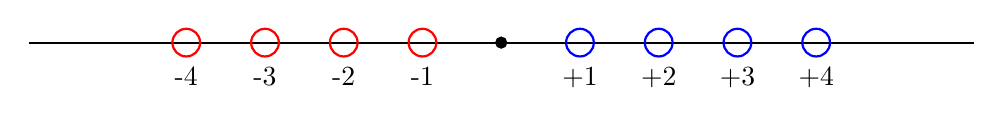
\begin{tikzpicture}
        \draw[thick] (-6,0) -- (6,0);
        \filldraw (0,0) circle (2pt);
        
        \foreach \x in {-4,-3,-2,-1} {
            \draw[red, thick] (\x,0) circle (5pt);
            \node[below] at (\x,-0.2) {\x};
	    }
        
        \foreach \x in {1,2,3,4} {
            \draw[blue, thick] (\x,0) circle (5pt);
            \node[below] at (\x,-0.2) {+\x};
 	    }
    \end{tikzpicture}
    \caption{ToyDF with 8 examples.}
    \label{fig:toydf}
\end{figure}

A structure like the one in Figure \ref{fig:toydf} allows for generating a dataset that, by construction, will lead to a fixed input graph $G$ for the minor embedding algorithm, called ToyGraph. 
For example, the data in figure \ref{fig:toydf} leads to the graph in figure \ref{fig:toydfgraph}.

\begin{figure}[H]
    \centering
    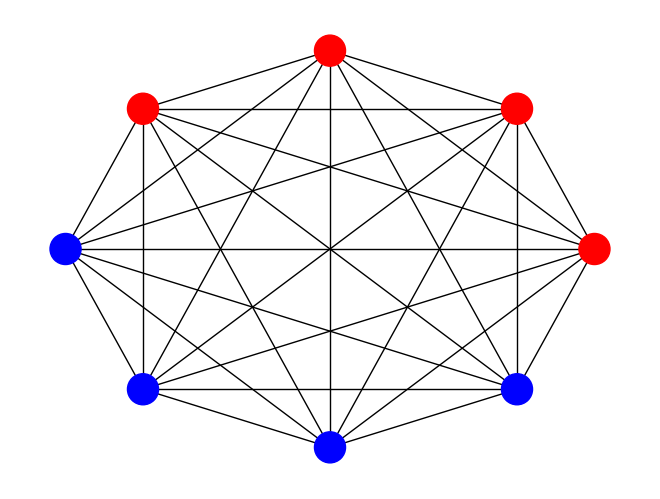
\includegraphics[scale=0.5]{figures/toygraph.png}
    \caption{Input graph $G$ for ToyDF of size $8$ and $UB=1$.}
    \label{fig:toydfgraph}
\end{figure}

The number of nodes of $G$ depends on only two factors:

\begin{itemize} 
	\item Equation \ref{eq:nodesnum}, where $\text{UB} = 1$ can be set to ensure that the number of nodes increases linearly with the number of examples; 
	\item The application or not of the pre-solving strategy, which, as discussed in Section \ref{sec:presolve}, doubles the number of required nodes when activated. 
\end{itemize}

SVMs generate a complete graph since each example is linked to each other. 
Although this structure is common in many optimization problems, it requires significant adjustments due to the low degree of the nodes in the Pegasus graph, as shown in Figure \ref{fig:QPU}.

\section{Results}\label{sec:qpu-res}

The search for minor embeddings for ToyGraph was conducted with various sizes of ToyDF. 
Given the heuristic nature of the minor embedding search, the algorithm needs a seed for the pseudorandom number generator to govern non-deterministic choices. 
According to the recommendations of \cite{random}, a good generator seed should be a prime number; therefore, the tests were repeated using the first 100 prime numbers.
The results shown in Table \ref{tab:scale} were obtained.

\begin{table}[H]
    \centering
    \begin{tabular}{ccc}
        \toprule
        Problem Nodes & Average Embedding Nodes & Average Time (s) \\
        \midrule
        \rowcolor{lightgray} 4 & 4 $\pm$ 0 & 0.3 \\
        6 & 8 $\pm$ 0 & 0.2 \\ 
        \rowcolor{lightgray} 8 & 11.1 $\pm$ 1.1 & 0.5 \\ 
        % 10 & 17.5 $\pm$ 0.9 & 0.6 \\ 
        12 & 20.4 $\pm$ 0.9 & 0.5 \\ 
        \rowcolor{lightgray} 16 & 32 $\pm$ 1.1 & 0.8 \\ 
        % 20 & 47.9 $\pm$ 2.4 & 0.12 \\ 
        24 & 63 $\pm$ 2.1 & 2.4 \\ 
        \rowcolor{lightgray} 32 & 102.2 $\pm$ 5.2 & 5.6 \\ 
        % 40 & 164 $\pm$ 8.4 & 9.9 \\ 
        48 & 218.8 $\pm$ 8 & 17.1 \\ 
        \rowcolor{lightgray} 64 & 372.7 $\pm$ 27.1 & 47.1 \\ 
        % 80 & 602 $\pm$ 34.3 & 92 \\ 
        96 & 801.5 $\pm$ 56.8 & 169.1 \\ 
        \rowcolor{lightgray} 128 & 1424.5 $\pm$ 95.8 & 376.5 \\ 
        % 160 & 2205.8 $\pm$ 182.8 & 703.1 \\ 
        192 & 1696.6 $\pm$ 118.7 & 468.9 \\ 
        \rowcolor{lightgray} 256 & 3067.1 $\pm$ 213.7 & 801.3 \\
        \bottomrule
    \end{tabular}
    \caption{Minor Embedding results on ToyDF}
    \label{tab:scale}
\end{table}

The columns in Table \ref{tab:scale} indicate: 
\begin{itemize} 
	\item \textbf{Problem Nodes}: The number of nodes in the original problem as in Figure \ref{fig:toydfgraph}; 
	\item \textbf{Average Embedding Nodes}: The number of nodes in the found embedding from $G$ to Pegasus; 
	\item \textbf{Average Time (s)}: The time, in seconds, taken to find the embedding. 
\end{itemize}

The rows in Table \ref{tab:scale} represent initial problems whose size is a power of two. 
Although this characteristic does not have significant consequences for the analysis, doubling the required number of nodes is not uncommon. This doubling can be due to:
\begin{itemize} 
	\item Use of pre-solving; 
	\item An increase in the upper bound of the $\alpha_i$ variables, which in an ideal (error-free) SVM scenario should be able to tend towards $+\infty$. 
\end{itemize}

Figure \ref{fig:scale_nodes} shows the number of QPU nodes required to find an embedding. 
The number of nodes required for the embedding is at least ten times the size of the input graph $G$.

For instance, a problem with 256 nodes, an insignificant dataset size compared to TweetDF, requires 3,000 qubits on the QPU. 
Given that current D-Wave QPUs have around 5,600 qubits, it is unlikely that an embedding will be found for larger problems.

\begin{figure}[H] 
	\centering 
	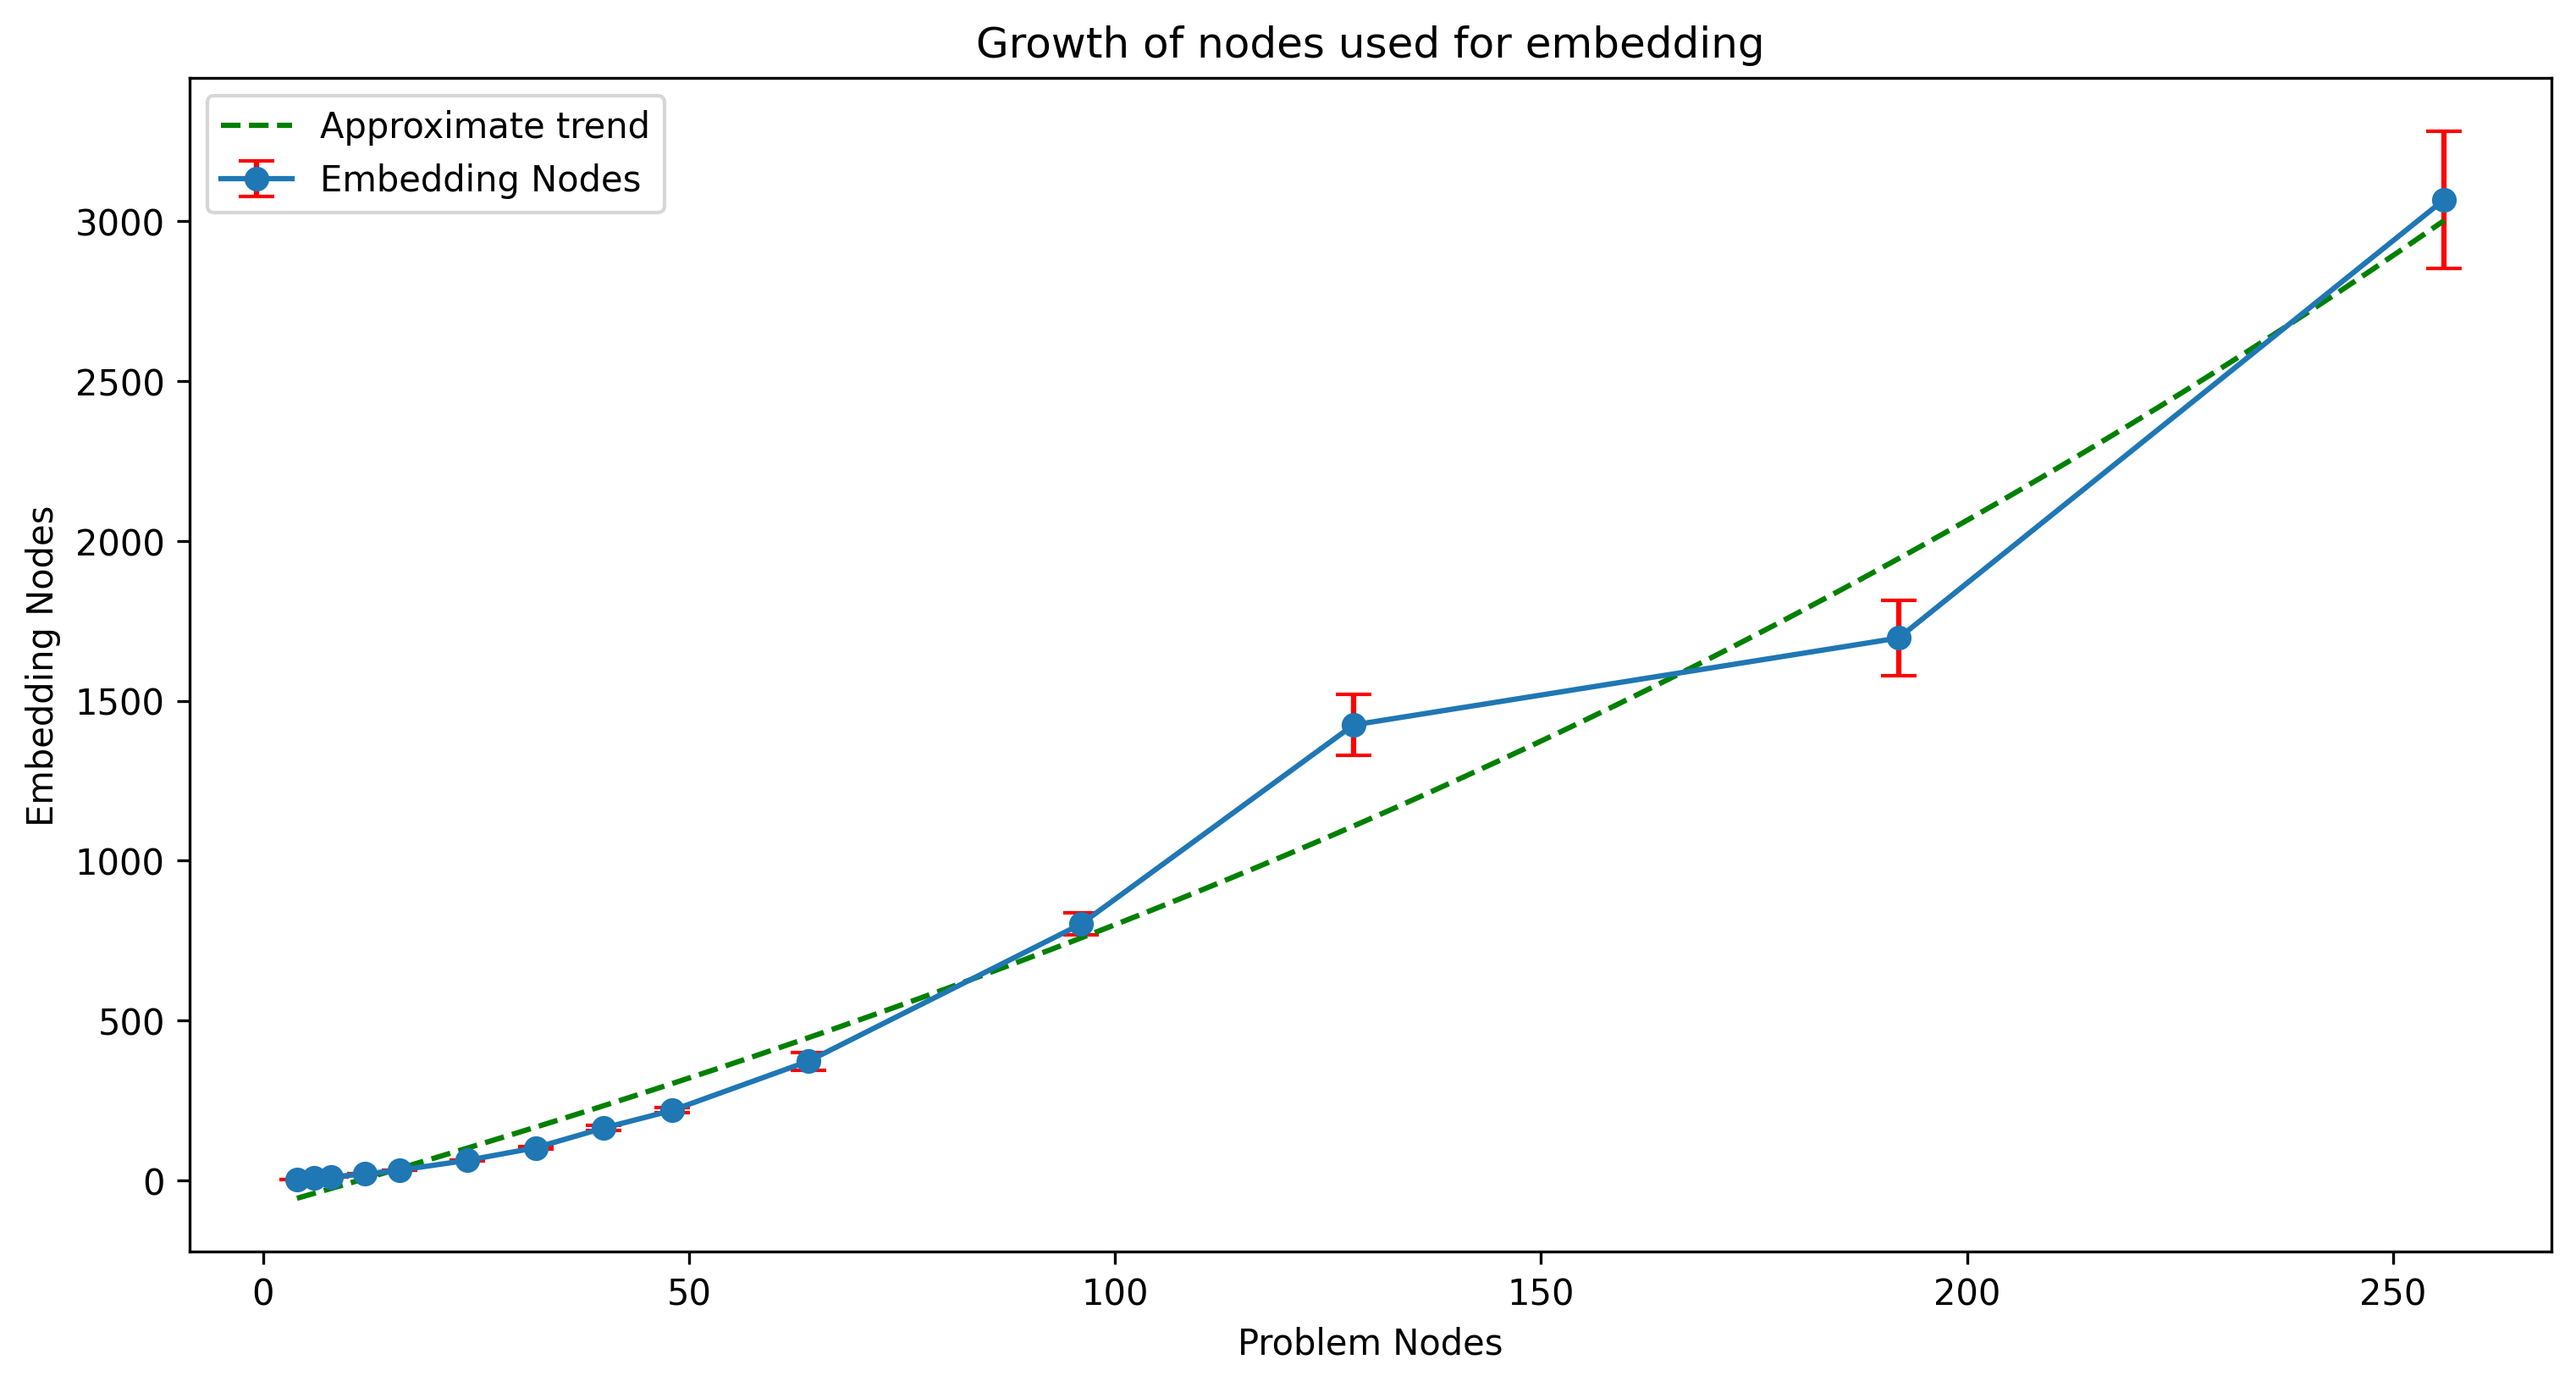
\includegraphics[width=\textwidth]{figures/scale_node.png} 
	\caption{Growth of nodes used for embedding.}
	\label{fig:scale_nodes}
\end{figure}

Figure \ref{fig:scale_time} shows the average time required to compute the embedding. 
The cost of the procedure significantly impacts performance, reaching 800 seconds for moderately sized problems.

Given that these times refer to a preprocessing operation, such high values are incompatible with the results recorded in Section \ref{sec:qsvm-performance}. 
In the case of the hybrid solver, the time recorded to compute the optimal solution with 4,096 examples and an upper bound of $\alpha = 255$ is less than the time required for the minor embedding search for problems with 128 nodes.

\begin{figure}[H] 
	\centering 
	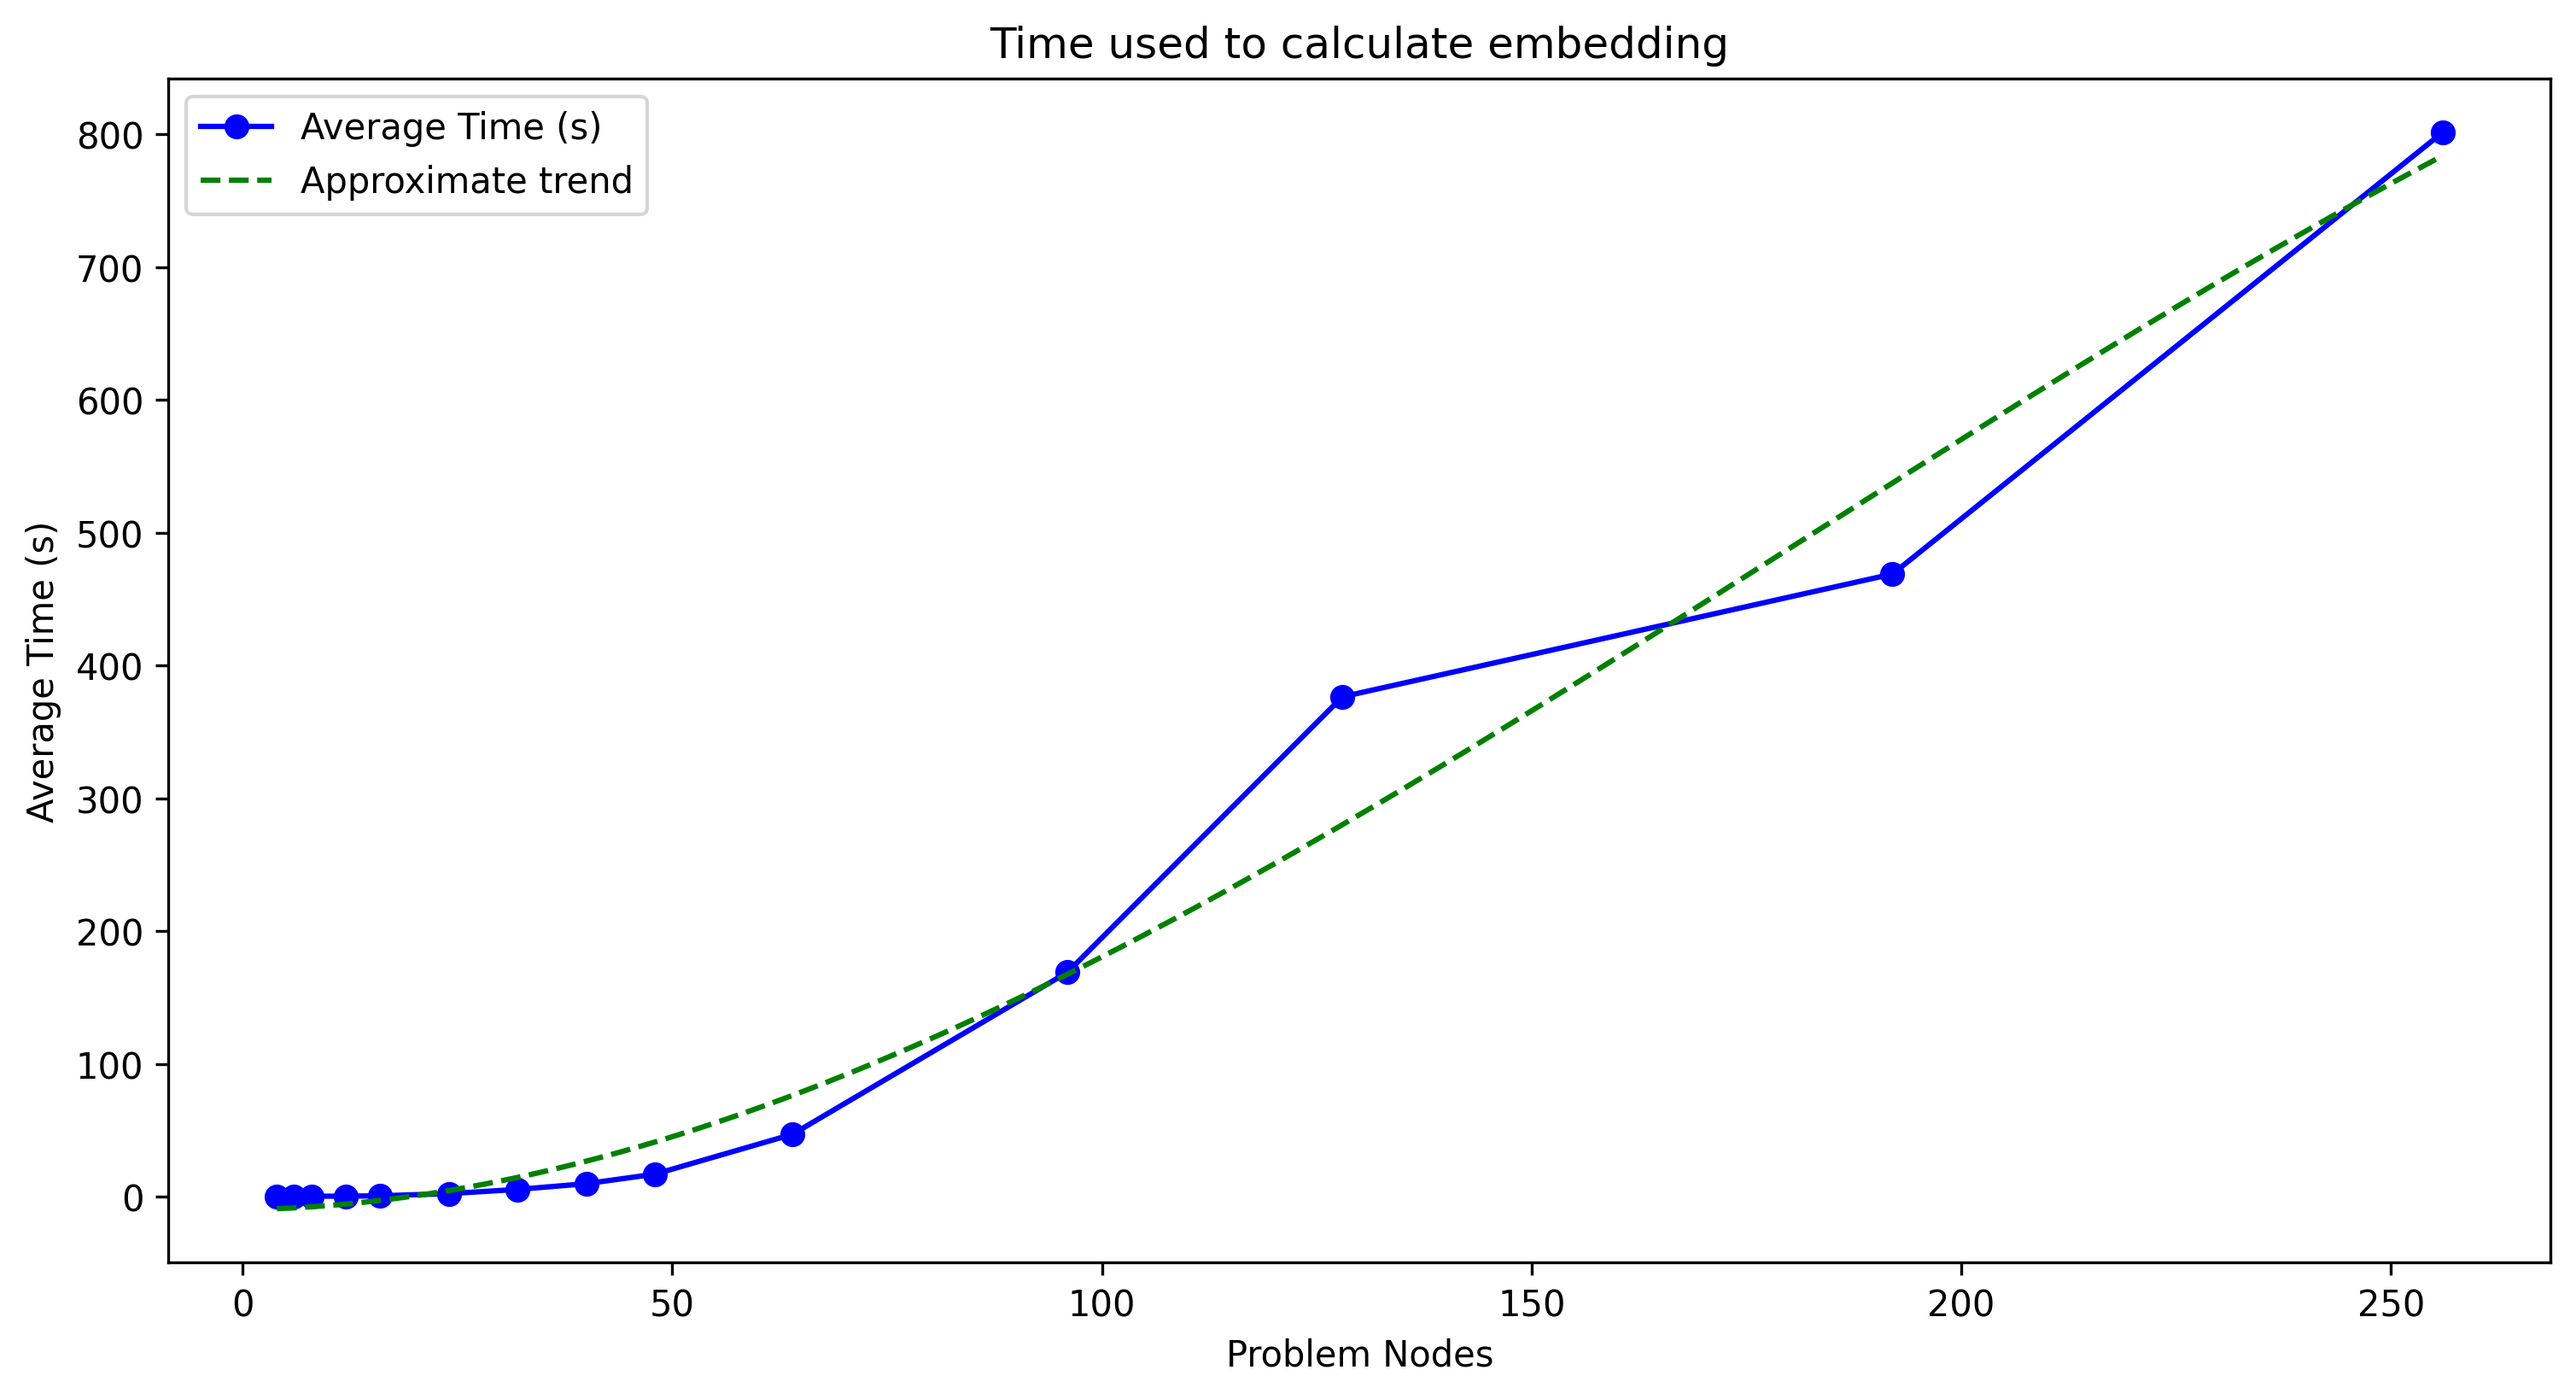
\includegraphics[width=\textwidth]{figures/scale_time.png} 	
	\caption{Time required to calculate embedding.} 
	\label{fig:scale_time}
\end{figure}

\subsection{QPU Solver vs. Hybrid Solver}

These findings strongly suggest that the direct use of the QPU is not a scalable alternative capable of solving problems beyond those currently addressed by classical computers.

The use of hybrid solvers is therefore a key step for the optimal utilisation of quantum annealing technology. 
It is therefore worth considering whether alternative hybrid solvers can be developed to further exploit the QPU and improve performance in problem-solving.

\part{Developing a Hybrid Solver}

\chapter{The underlying idea of a hybrid solver}

\chapter{QUBO Splitting Algorithm}

Following the theoretical discussion on the feasibility of the algebraic partitioning method in Section \ref{sec:prop}, this chapter provides an account of its implementation, which is one of the outcome of the work. 
Chapter \ref{sec:qsplitres} will present the results obtained from testing the procedures outlined.

\section{QUBO Utility Class}

Thus far, QUBO problems have been presented and analyzed in matrix form or as the equivalent produced equation. 
While matrices can represent these problems, the coefficient matrix $Q$ is often sparse, i.e. it contains many zero values relative to the total number of matrix cells.

Since a QUBO problem is characterised by an upper triangular matrix, the maximum number of non-zero values is $n(n+1)/2$, where $n$ is the dimension of the $Q$ matrix. 
This implies, by definition, at least $n(n-1)/2$ zero values. Since QUBO problem information must be transmitted between different computers for processing, D-Wave has changed the representation format to eliminate redundant information.

To achieve this, instead of matrices, \textsc{HashMap}s are used, where the key is the pair representing the position in the matrix $(\text{row}, \text{col})$, and the value corresponds to the matrix coefficient at that cell. 
In this way, all zero values are ``discarded'', representing only the relevant information that characterizes the problem.

To operate effectively, it is necessary to maintain a dual representation of the QUBO problem: 
\begin{enumerate} 
	\item A matrix form for performing algebraic operations; 
	\item A minimal representation for transmitting the problem to D-Wave quantum solvers. 
\end{enumerate}

For this reason, a support class \texttt{QUBO} was developed during this thesis to manage the consistency between the two representations automatically. 
The \texttt{QUBO} class is responsible for: 
\begin{itemize} 
	\item Maintaining a copy of the matrix representation; 
	\item Maintaining a copy of the compact representation; 
	\item Storing a set of solutions for the problem, if provided; 
	\item Keeping track of the variables associated with the rows and col\-umns of the matrix. 
    This additional information is crucial because, during decomposition, the symbolic names of variables could be lost, leading to meaningless assignments.
\end{itemize}

The available methods are responsible for:
\begin{itemize} 
	\item Converting the problem from one representation to the other; 
	\item Verifying whether the matrix is upper triangular; if not, it is converted using the LU algorithm\cite{LU}.
\end{itemize}

\section{\texttt{QSplitSampler} Implementation}

The main points of the implementation are outlined below, along with an explanatory example; the complete code for \texttt{QSplitSampler} is available on GitHub\footnote{\url{https://github.com/TheFlonet/qsvm4sentanalysis/tree/main/subqubo}}.

\subsection{Main Method}

\texttt{QSplitSampler} distinguishes the execution of the main block into two categories: 
\begin{itemize} 
	\item Small-scale problems, or generally manageable-sized problems; 
	\item Problems that require partitioning. 
\end{itemize}

In the first case, the algorithm uses the QPU to solve QUBO instances where the problem size is less than \texttt{CUT\_DIM}, the cut-off size that distinguishes a manageable problem from one that cannot be addressed directly.

In the second case, the QUBO problem is partitioned using the \texttt{split\_problem} method, presented in Section \ref{sec:split}. 
Once the solutions are computed, they are aggregated using \texttt{aggregate\_solutions}, Section \ref{sec:aggr}.

The reference code can be found in Listing \ref{code:main}.

\begin{lstlisting}[language=Python, caption=QSplitSampler main function, label=code:main]
def QSplitSampler(qubo: QUBO, dim: int) -> QUBO:
    if dim <= CUT_DIM:
        res = SAMPLER.sample_qubo(qubo.qubo_dict, num_reads=10)
        qubo.solutions = res[min(res.energy)]
        return qubo

    sub_problems = split_problem(qubo, dim)
    for i, q in enumerate(sub_problems):
        sub_problems[i] = QSplitSampler(q, dim // 2)
    return aggregate_solutions(sub_problems, qubo)
\end{lstlisting}

For example, suppose setting the parameters of \texttt{QSplitSampler} as follows:
\begin{itemize}
    \item The problems solved directly via QPU are composed of two variables;
    \item The QPU returns four assignments;
    \item At the end of each recursive step, only the three best solutions are retained.
\end{itemize}

A starting QUBO problem could be:

\begin{equation}
    \begin{bmatrix}
        x_1 & x_2 & x_3 & x_4
    \end{bmatrix}
    \begin{bmatrix}
        1 & 2 & 3 & 4 \\
        0 & 5 & 6 & 7 \\
        0 & 0 & 8 & 9 \\
        0 & 0 & 0 & 10 \\
    \end{bmatrix}
    \begin{bmatrix}
        x_1 \\
        x_2 \\
        x_3 \\
        x_4
    \end{bmatrix}
    \label{eq:example_full}
\end{equation}

\subsection{Split Method}\label{sec:split}

The partitioning methodology follows the approach described in Section \ref{sec:prop}, where the matrix describing the QUBO problem is divided into four parts, with only three being returned, as one is zero by definition and does not contribute to the solution.

The order in which the new subproblems are returned is as follows: 
\begin{itemize} 
	\item The $\operatorname{UL}$ problem, corresponding to the top-left subproblem, it operates on the first half of the optimization variables; 
	\item The $\operatorname{UR}$ problem, the top-right sub-matrix portion, operating on both partitions of the variables; 
	\item The $\operatorname{BR}$ problem, the bottom-right sub-matrix portion, operates on the second half of the optimization variables. 
\end{itemize}

The following subproblems are obtained from \eqref{eq:example_full}:
\begin{itemize}
    \item $\operatorname{UL}$
    \begin{equation}
        \begin{bmatrix}
            x_1 & x_2
        \end{bmatrix}
        \begin{bmatrix}
            1 & 2 \\
            0 & 5
        \end{bmatrix}
        \begin{bmatrix}
            x_1 \\
            x_2
        \end{bmatrix}
        \label{eq:exampleUL}
    \end{equation}
    \item $\operatorname{UR}$
    \begin{equation}
        \begin{bmatrix}
            x_1 & x_2
        \end{bmatrix}
        \begin{bmatrix}
            3 & 4 \\
            6 & 7
        \end{bmatrix}
        \begin{bmatrix}
            x_3 \\
            x_4
        \end{bmatrix}
        \label{eq:exampleUR}
    \end{equation}
    \item $\operatorname{BR}$
    \begin{equation}
        \begin{bmatrix}
            x_3 & x_4
        \end{bmatrix}
        \begin{bmatrix}
            8 & 9 \\
            0 & 10
        \end{bmatrix}
        \begin{bmatrix}
            x_3 \\
            x_4
        \end{bmatrix}
        \label{eq:exampleBR}
    \end{equation}
\end{itemize}

Although all matrix portions are converted to be upper triangular, problem obtained by $\operatorname{UR}$ like \eqref{eq:exampleUR} is, by definition, not in QUBO form. 
This is because it operates on both partitions of the optimization variables, meaning $X^T \neq X$.

The compact representation required by D-Wave allows the solver to determine the problem dimensions automatically. 
Therefore, the problem solved in this case does not take the form shown in Equation \eqref{eq:ur}.
The subproblem \eqref{eq:exampleUR}, for example, is shaped in \eqref{eq:realur}.

\begin{equation}
    \begin{bmatrix}
        x_1 & x_2 & x_3 & x_4
    \end{bmatrix}
    \begin{bmatrix}
        0 & 0 & 8 & 9 \\
        0 & 0 & 0 & 10 \\
        0 & 0 & 0 & 0 \\
        0 & 0 & 0 & 0 
    \end{bmatrix}
    \begin{bmatrix}
        x_1 \\
        x_2 \\
        x_3 \\
        x_4 
    \end{bmatrix}
    \label{eq:realur}
\end{equation}

That is, the subproblem is ``embedded'' in a zero matrix with dimensions equal to those of the original problem. 
This operation seems to negate the dimensionality reduction of the QUBO problem; however, the underlying representation of the problem remains sufficiently small to allow its resolution like the other two sub-matrices.

\subsection{Aggregation Method}\label{sec:aggr}

Once the subproblems are solved, the results must be aggregated to provide a complete solution to the problem.

\paragraph{UL-BR aggregation} Since these subproblems operate on different partitions of the variables, a Cartesian product of their partial assignments is performed to consider all possible combinations. 

Referring $S_{\operatorname{UL}}$, Equation \eqref{eq:s_ul}, as the solutions of \eqref{eq:exampleUL}, and $S_{\operatorname{BR}}$, Equation \eqref{eq:s_br}, as the solutions of \eqref{eq:exampleBR}, from their Cartesian product the solutions given in \eqref{eq:ulrb} are obtained.

\begin{equation}
    S_{\operatorname{UL}} =\{\{x_1=0,x_2=0\}, \{x_1=1,x_2=0\}, \{x_1=0,x_2=1\}\}
    \label{eq:s_ul}
\end{equation}

\begin{equation}
    S_{\operatorname{BR}} =\{\{x_3=0,x_4=0\}, \{x_3=1,x_4=0\}\}
    \label{eq:s_br}
\end{equation}

\begin{equation}
    S_{\operatorname{UL}-\operatorname{BR}}=\left[
    \begin{array}{c}
        \{x_1=0,x_2=0,x_3=1,x_4=0\} \\
        \{x_1=1,x_2=0,x_3=0,x_4=0\} \\
        \{x_1=1,x_2=0,x_3=1,x_4=0\} \\
        \{x_1=0,x_2=1,x_3=0,x_4=0\} \\
        \{x_1=0,x_2=1,x_3=1,x_4=0\} \\
        \{x_1=0,x_2=0,x_3=0,x_4=0\}
    \end{array}
    \right]
    \label{eq:ulrb}
\end{equation}

\paragraph{UR contribution} For each assignment of $S_{\operatorname{UL}-\operatorname{BR}}$ \eqref{eq:ulrb} the closest assignment of $S_{\operatorname{UR}}$, Equation \eqref{eq:ursol}, is searched.

\begin{equation}
    S_{\operatorname{UR}}=\left[
        \begin{array}{c}
            \{x_1=0,x_2=0,x_3=0,x_4=0\},\\ 
            \{x_1=1,x_2=0,x_3=0,x_4=0\},\\
            \{x_1=0,x_2=1,x_3=0,x_4=0\},\\
            \{x_1=0,x_2=0,x_3=1,x_4=0\}
        \end{array}
        \right]
        \label{eq:ursol}
\end{equation}

The following pairs of assignments are obtained:
\begin{itemize}
    \item $S_1 = \langle S_{\operatorname{UL}-\operatorname{BR}}[1], S_{\operatorname{UR}}[4]\rangle$, with no conflicting variables;;
    \item $S_2 = \langle S_{\operatorname{UL}-\operatorname{BR}}[2], S_{\operatorname{UR}}[2]\rangle$, with no conflicting variables;;
    \item $S_3 = \langle S_{\operatorname{UL}-\operatorname{BR}}[3], S_{\operatorname{UR}}[2]\rangle$, conflicting on the variable $x_3$;
    \item $S_4 = \langle S_{\operatorname{UL}-\operatorname{BR}}[4], S_{\operatorname{UR}}[3]\rangle$, with no conflicting variables;;
    \item $S_5 = \langle S_{\operatorname{UL}-\operatorname{BR}}[5], S_{\operatorname{UR}}[3]\rangle$, conflicting on the variable $x_3$;
    \item $S_6 = \langle S_{\operatorname{UL}-\operatorname{BR}}[6], S_{\operatorname{UR}}[1]\rangle$, with no conflicting variables;.
\end{itemize}

\paragraph{Final answer set} The resolution of conflicting assignments is dealt with in detail in Section \ref{sec:qsearch}, once assignments without conflicting variables have been obtained, the value of the objective function $X^TQX$ is calculated and the $k$ assignments with the lowest value are kept.

Solving the conflicts in $S_3$ and $S_5$, the final assignments produced by \texttt{QSplitSampler} are:
\begin{itemize}
    \item $S_1$, with an objective function value of 8;
    \item $S_2 = S_3$, with objective function value of 1;
    \item $S_4 = S_5$, with objective function value of 5;
    \item $S_6$, with objective function value of 0.
\end{itemize}

The resulting assignments produced for the problem \eqref{eq:example_full} are then $S_6$, $S_2$ and $S_4$

\subsection{Quantum Local Search}\label{sec:qsearch}

Conflicting assignments can be resolved using various search methodologies, including: 
\begin{enumerate} 
	\item Brute-force; 
	\item Local search; 
	\item Extraction of a new QUBO problem. 
\end{enumerate}

Brute-force was initially implemented, but for non-trivial problems, the number of assignments to test led to intractable issues.

Local search techniques might be promising, but it would go against the principle underlying the development of \texttt{QSplitSampler}, which is to maximize the use of the QPU.

For these reasons, the most reasonable option was to assess the feasibility of using the QPU to resolve conflicting assignments.

\begin{lstlisting}[language=Python, caption=QUBO extractor function, label=code:qsearch]
def q_search(df: pd.DataFrame, qubo: QUBO) -> pd.DataFrame:
    for i, row in df.iterrows():
        no_energy = row.drop(energy)

        nans = no_energy[np.isnan(no_energy)]
        qubo_nans = defaultdict(int)
        for row_idx in nans.index:
            for col_idx in nans.index:
                val = qubo.qubo_dict.get((row_idx, col_idx), 0)
                qubo_nans[(row_idx, col_idx)] = val
        nans_sol = SAMPLER.sample_qubo(qubo_nans, num_reads=10)
        nans_sol = nans_sol.to_pandas_dataframe()
                           .sort_values(by=energy, 
                                        ascending=True).iloc[0]
        df.loc[i, nans.index] = nans_sol.drop(energy)
        df.loc[i, energy] += nans_sol.energy

    return df
\end{lstlisting}

The underlying idea of the proposed in Listing \ref{code:qsearch} search mechanism is to extract a subproblem focusing on the rows and columns associated with the conflicting variables. 
Once extracted and converted in upper triangular, the subproblem can be resolved again on the QPU.

In the problem \eqref{eq:example_full} the only variable that generates conflicting assignments is $x_3$, so the row and column relating to that variable must be extracted from the matrix $Q$.
Since there is only one value, the QUBO formulation reduces to $\min 8x_3^2$, which is minimised by assigning $x_3$ the value zero.

Unlike the method discussed in Section \ref{sec:split}, this search approach does not guarantee a specific size for the resulting problem.
Because in the case of complementary assignments, for example like $\{x_1=1,x_2=0,x_3=1,x_4=0\}$ and $\{x_1=0,x_2=1,x_3=0,x_4=1\}$, the number of conflicting variables equals the total number of variables considered. 

Experimentally, the number of variables with conflicting assignments remained small enough to allow resolution via the QPU.

\chapter{Effectiveness of QUBO splitting}\label{sec:qsplitres}

The following chapter analyzes the effectiveness of \texttt{QSplitSampler} when applied to ``real'' problems.

The analysis compares \texttt{QSplitSampler} with D-Wave's solver that directly utilizes the QPU, namely \texttt{QPUSampler}.
The data collected focuses on:
\begin{itemize}
    \item The quality of the solution produced, specifically how close the assignment is to the global optimum;
    \item The time required for the resolution, considering both time spent on the QPU and CPU.
\end{itemize}

Section \ref{sec:maxcut} examines a specific instance of the Maximum-Cut Problem (MCP).
The selected instance can be easily visualised and has some desirable features for evaluating the performance of \texttt{QSplitSampler} under ``adverse'' conditions.

Section \ref{sec:qsplittest} analyzes a series of randomly generated problems to evaluate not only the solution quality but, more importantly, the time advantage of \texttt{QSplitSampler} compared to \texttt{QPUSampler} by assessing whether increased QPU usage results in a shorter overall time to compute the solution.

\section{Test case: Maximum-Cut Problem}\label{sec:maxcut}

To evaluate \texttt{QSplitSampler} effectiveness it is natural to set a controlled environment, as opposed to the real scenario provided by sentiment analysis applications.
The real scenario selected is represented by the solution to instances of MCP, reduced to QUBO. 

Motivations to choose MCP are:
\begin{itemize}
    \item It is straightforward to manually construct problems with a specified number of edges and nodes;
    \item It is a problem that can be reformulated easily in QUBO form;
    \item It exhibits symmetric solutions, meaning that the assignment of binary variables or their complementary assignment yields the same objective function value.
    Therefore, the optimal solution to MCP will never be unique, as there will always be at least two optimal assignments.
\end{itemize}

\subsection{Maximum-Cut}

MCP involves dividing the vertices of a graph into two subsets, $S$ and $T$, such that the number of edges between nodes in $S$ and nodes in $T$ is maximized.

Consider a graph like the one in Figure \ref{fig:maxcut}. 
Subset $S$ consists of the white nodes, and subset $T$ consists of the black nodes. 
Figure \ref{fig:maxcutset} highlights all and only the edges between $S$ and $T$.

\begin{figure}[H]
    \centering
    \begin{subfigure}[b]{0.48\textwidth}
        \centering
        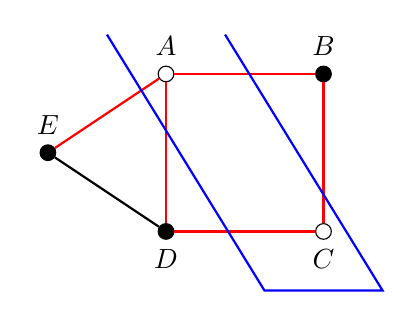
\begin{tikzpicture}
            \node[circle, fill=white, draw=black, inner sep=2pt, label=above:$A$] (A) at (0,2) {};
            \node[circle, fill=black, draw=black, inner sep=2pt, label=above:$B$] (B) at (2,2) {};
            \node[circle, fill=white, draw=black, inner sep=2pt, label=below:$C$] (C) at (2,0) {};
            \node[circle, fill=black, draw=black, inner sep=2pt, label=below:$D$] (D) at (0,0) {};
            \node[circle, fill=black, draw=black, inner sep=2pt, label=above:$E$] (E) at (-1.5,1) {};
            
            \draw[red, thick] (A) -- (B);
            \draw[red, thick] (B) -- (C);
            \draw[red, thick] (C) -- (D);
            \draw[red, thick] (D) -- (A);
            \draw[red, thick] (A) -- (E);
            \draw[black, thick] (E) -- (D);
        
            \draw[blue, thick] ($(A)+(0.75,0.5)$) -- ($(C)+(0.75,-0.75)$) -- ($(C)+(-0.75,-0.75)$) -- ($(A)+(-0.75,0.5)$);
        \end{tikzpicture}
        \caption{Maximum-Cut example graph.}
        \label{fig:maxcut}
    \end{subfigure}
    \hfill
    \begin{subfigure}[b]{0.48\textwidth}
        \centering
        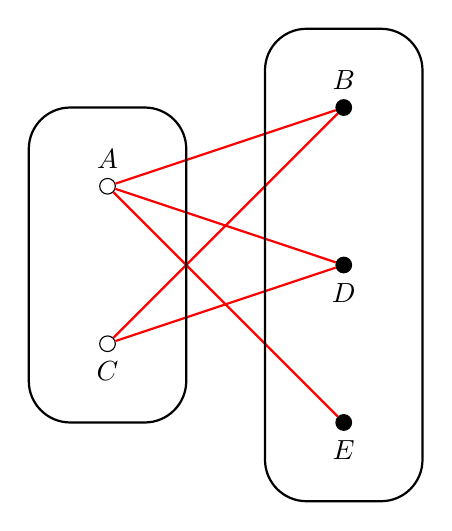
\begin{tikzpicture}
            \node[circle, fill=white, draw=black, inner sep=2pt, label=above:$A$] (A) at (0,3) {};
            \node[circle, fill=white, draw=black, inner sep=2pt, label=below:$C$] (C) at (0,1) {};
            
            \node[circle, fill=black, draw=black, inner sep=2pt, label=above:$B$] (B) at (3,4) {};
            \node[circle, fill=black, draw=black, inner sep=2pt, label=below:$D$] (D) at (3,2) {};
            \node[circle, fill=black, draw=black, inner sep=2pt, label=below:$E$] (E) at (3,0) {};
            
            \draw[red, thick] (A) -- (B);
            \draw[red, thick] (A) -- (E);
            \draw[red, thick] (A) -- (D);
            \draw[red, thick] (C) -- (B);
            \draw[red, thick] (C) -- (D);
            
            \draw[black, thick, rounded corners=15pt] (-1,0) rectangle (1,4);
            \draw[black, thick, rounded corners=15pt] (2,-1) rectangle (4,5);
        \end{tikzpicture}
        \caption{Rearranged graph in $S$ and $T$.}
        \label{fig:maxcutset}
    \end{subfigure}
    \caption{Maximum-Cut (a) and subdivision into subsets (b).}
\end{figure}

\paragraph{Desired Characteristics} In the case illustrated in Figure \ref{fig:maxcut}, it is easily verifiable that it is impossible to find an assignment of $S$ and $T$ that produces more than five edges.

However, the solution is not unique. 
Associating $1$ with the white nodes and $0$ with the black nodes, two five-edge solutions are: 
\begin{itemize}
    \item $\{A=1,B=0,C=1,D=0,E=0\}$,
    \item $\{A=0,B=1,C=0,D=1,E=1\}$.
\end{itemize}

The non-uniqueness of the solution presents a challenge during the optimization process, as different sections of the problem might guide towards complementary assignments, leading to inconsistent aggregated results when, recalling Section \ref{sec:split}, a QUBO problem is splitted, possibly recursively, into smaller instances.

\subsection{Results}

\texttt{QSplitSampler} was configured to solve problems using \texttt{QPUSampler} that only consider two variables. 
Since the initial problem size consists of eight variables, the submatrices considered for direct resolution have a size equal to $\frac{2^2}{8^2} = \frac{1}{16}$ of the original problem.

In this case, partitioning is unnecessary, as the QPU can directly solve problems of this size. 
The utility of this experiment lies in providing an initial measure of error.

In particular, the instance of MCP under consideration is represented in Figure \ref{fig:maxcut_test}.
The graph represents a problem with eight nodes, corresponding to eight binary variables.

\begin{figure}[H]
    \centering
    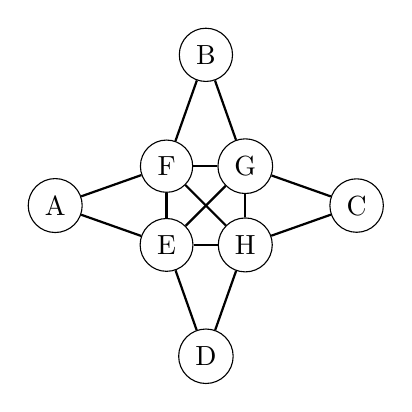
\begin{tikzpicture}
        \node[circle, draw=black] (A) at (0,1.914) {A};
        \node[circle, draw=black] (B) at (1.914,3.828) {B};
        \node[circle, draw=black] (C) at (3.828,1.914) {C};
        \node[circle, draw=black] (D) at (1.914,0) {D};
        \node[circle, draw=black] (E) at (1.414,1.414) {E};
        \node[circle, draw=black] (F) at (1.414,2.414) {F};
        \node[circle, draw=black] (G) at (2.414,2.414) {G};
        \node[circle, draw=black] (H) at (2.414,1.414) {H};

        \draw[black, thick] (A) -- (E);
        \draw[black, thick] (A) -- (F);
        \draw[black, thick] (B) -- (F);
        \draw[black, thick] (B) -- (G);
        \draw[black, thick] (C) -- (G);
        \draw[black, thick] (C) -- (H);
        \draw[black, thick] (D) -- (H);
        \draw[black, thick] (D) -- (E);
        \draw[black, thick] (E) -- (F);
        \draw[black, thick] (E) -- (H);
        \draw[black, thick] (E) -- (G);
        \draw[black, thick] (F) -- (G);
        \draw[black, thick] (F) -- (H);
        \draw[black, thick] (H) -- (G);
    \end{tikzpicture}
    \caption{Graph used to test Maximum-Cut.}
    \label{fig:maxcut_test}
\end{figure}

Following the examples provided by D-Wave itself \cite{maxcut-dwave}, it is possible to convert the graph in Figure \ref{fig:maxcut_test} into a QUBO formulation, resulting in the upper triangular matrix shown in the matrix \eqref{eq:maxcutQUBO}.

\begin{equation}
    \begin{array}{c|*{8}{c}}
          & A  & B  & C  & D  & E  & F  & G  & H  \\
        \hline
        A & -2 & 0  & 0  & 0  & 2  & 2  & 0  & 0  \\
        B &    & -2 & 0  & 0  & 0  & 2  & 2  & 0  \\
        C &    &    & -2 & 0  & 0  & 0  & 2  & 2  \\
        D &    &    &    & -2 & 2  & 0  & 0  & 2  \\
        E &    &    &    &    & -5 & 2  & 2  & 2  \\
        F &    &    &    &    &    & -5 & 2  & 2  \\
        G &    &    &    &    &    &    & -5 & 2  \\
        H &    &    &    &    &    &    &    & -5 \\
    \end{array}
    \label{eq:maxcutQUBO}
\end{equation}

Solving the problem \eqref{eq:maxcutQUBO} yields the results given in Table \ref{tab:maxcut}.

\begin{table}[H]
    \centering
    \begin{tabular}{cccc}
        \toprule
        \multicolumn{2}{c}{\texttt{QSplitSampler}} & \multicolumn{2}{c}{\texttt{QPUSampler}} \\
        Time (s) & Solution & Time (s) & Solution \\
        \midrule
        18.15 & 0.8 & 5.02 & 0        
    \end{tabular}
    \caption{\texttt{QSplitSampler} executed on \eqref{eq:maxcutQUBO}.}
    \label{tab:maxcut}
\end{table}

The time required to process the problem is expressed in seconds and includes the following components: 
\begin{itemize} 
    \item Processing on the CPU, which, in the case of a direct solution, consists only of initializing the data structure; 
    \item Network transfer, to send the problem to quantum solvers;
    \item Processing on the QPU, to produce the solution. 
\end{itemize}

The solution is presented by normalizing the values within the range $[0, 1]$. 
Since these are minimization problems, $0$ corresponds to the optimal solution.

\paragraph{Time Analysis} The time required to solve MCP on the graph in Figure \ref{fig:maxcut_test} with \texttt{QSplitSampler} is 3.6 times greater than that of a direct resolution. 
In detail, three main components can be identified that contribute to the time spent on classical machines:
\begin{itemize}
    \item Calculation of the minor embedding;
    \item Partitioning algorithm and aggregation of the subproblems;
    \item Time required to send the subproblems generated to \texttt{QPUSampler}.
\end{itemize}
The last of these components represents the dominant factor that causes \texttt{QSplitSampler} to perform worse than \texttt{QPUSampler} for small-sized problems.
Since, it is necessary to transmit the data to D-Wave's cloud infrastructure, wait for processing, and then forward the result, this computational overhead might become marginal for instances where quantum acceleration is substantial, but it significantly impacts the resolution of ``small'' problems.

\paragraph{Quality of Results} From a performance perspective, \texttt{QSplitSampler} produced results that were significantly worse compared to direct resolution. 
However, it is important to contextualize these results.

\texttt{QSplitSampler} provided a response of $0.8$, a value closer to the maximum assignment than to the minimum. 
For the tests conducted, this represents an upper bound on the error made in producing a solution. 
The poor quality of the response could be due to multiple optimal solutions, all equivalent from an algorithmic standpoint but leading to final assignments that are inconsistent with the original problem.

\section{Extensive testing}\label{sec:qsplittest}

To evaluate the performance of \texttt{QSplitSampler} in a broader context than that described in Section \ref{sec:maxcut}, random problems were generated using D-Wave's libraries. 
The problems considered represent complete graphs, and while they do not represent SVMs, they preserve their structure and information density.

Working with complete graphs increases the likelihood of having multiple optimal assignments. 
Intuitively, this occurs because the problem has more data to combine to converge to the same objective function value.

\subsection{64 and 128 Variables Problems}\label{sec:multivar}

Using D-Wave's libraries to generate complete graphs, problems with $64$ and $128$ variables were solved, with the results reported in Tables \ref{tab:64var} and \ref{tab:128var}, respectively.

The table columns provide the following information, with all times expressed in seconds: 
\begin{enumerate}
    \item \texttt{QSplitSampler}
    \begin{enumerate}
        \item \emph{Cut Dim}: Number of variables handled by the subproblem sent directly to \texttt{QPUSampler};
        \item \emph{CPU \& QPU time}: Represented as \emph{CPU time - QPU time};
        \item \emph{Solution};
    \end{enumerate}
    \item \texttt{QPUSampler}
    \begin{enumerate}
        \item \emph{CPU \& QPU time}: Represented as \emph{CPU time - QPU time};
        \item \emph{Solution}.
    \end{enumerate}
\end{enumerate}

\begin{itemize}
    \item \emph{CPU time}: The time required by \texttt{QSplitSampler} to produce a solution, which includes:
    \begin{itemize}
        \item The time take for minor embedding computation;
        \item The time for network transfer to D-Wave's cloud infrastructure;
        \item The time spent on classical architecture processing (partition and aggregation of results).
    \end{itemize}
    \item \emph{QPU time}: The time spent on the QPU;
    \item \emph{Solution} is the value of the best solution, normalized to $[0, 1]$.
\end{itemize}

\subsubsection{Results}

Referring to the first row of Table \ref{tab:64var}, it can be observed that the total time required to provide the solution using \texttt{QSplitSampler} is approximately seven times greater than that required by \texttt{QPUSampler}.
The increased time is due to the number of subproblems processed, a topic that will be discussed in detail in Section \ref{sec:subproblemcount}.

As well as the time spent on the CPU, the time spent on the QPU increases significantly, by a factor of 16.5, where \texttt{QSplitSampler} takes 0.33 seconds compared to 0.02 seconds for \texttt{QPUSampler}.

However, the quality of the solution produced is unacceptable; while \texttt{QPUSampler} reaches the global optimum, \texttt{QSplitSampler} deviates significantly, yielding a value of 0.45.

\begin{table}[H]
    \centering
    \begin{tabular}{ccc|cc}
        \toprule
        \multicolumn{3}{c}{\texttt{QSplitSampler}} & \multicolumn{2}{c}{\texttt{QPUSampler}} \\
        Cut Dim & CPU \& QPU time & Solution & CPU \& QPU time & Solution \\
        \midrule
        2 & 154.23 - 0.33 & 0.45 & 22.06 - 0.02 & 0 \\
        4 & 73.76 - 0.25 & 0.42 & 21.41 - 0.02 & 0 \\
        8 & 40.51 - 0.17 & 0.43 & 36.54 - 0.02 & 0 \\
        16 & 24.6 - 0.10 & 0.42 & 37.87 - 0.02 & 0 \\
        32 & 20.68 - 0.05 & 0.33 & 16.67 - 0.02 & 0 \\
        \bottomrule
    \end{tabular}
    \caption{Results for problems with 64 variables.}
    \label{tab:64var}
\end{table}

\begin{table}[H]
    \centering
    \begin{tabular}{ccc|cc}
        \toprule
        \multicolumn{3}{c}{\texttt{QSplitSampler}} & \multicolumn{2}{c}{\texttt{QPUSampler}} \\
        Cut Dim & CPU \& QPU time & Solution & CPU \& QPU time & Solution \\
        \midrule
        2 & 414.42 - 0.45 & 0.36 & 144.29 - 0.02 & 0 \\
        4 & 169.13 - 0.35 & 0.47 & 183.23 - 0.02 & 0 \\
        8 & 95.89 - 0.25 & 0.5 & 168.34 - 0.02 & 0 \\
        16 & 63.83 - 0.17 & 0.52 & 106.02 - 0.02 & 0 \\
        32 & 45.42 - 0.1 & 0.42 & 143.97 - 0.02 & 0 \\
        \bottomrule
    \end{tabular}
    \caption{Results for problems with 128 variables.}
    \label{tab:128var}
\end{table}

In both tables, the quality of the solution produced deviates significantly from the optimum, deteriorating between 25\% and 50\%. 
Furthermore, the lower limit of the error committed seems to increase as the problem size increases, stabilising at around 35\%.

Despite the suboptimal results, \texttt{QSplitSampler} maintains the desired behaviour regarding QPU usage. 
All reported values exceed 0.1 seconds, three times higher than the use of D-Wave's hybrid solver (Section \ref{sec:qpuusage}) for significantly larger problems.

However, despite the significant increase in the quantum component used to find the solution, the time required to transmit all the subproblems and aggregate the results remains dominant.

Based on the results obtained, the following key considerations emerge: 
\begin{itemize} 
    \item The effectiveness of maximizing QPU usage as a resolution strategy; 
    \item The evident increase in solution time as \emph{cut dim} decreases. 
\end{itemize}

\paragraph{Performance} Although no clear relationship emerges between the parameters \texttt{QSplitSampler} and the quality of the solution produced, it is evident that an error of at least 25\% for small-sized problems is not acceptable. 
The poor performance is likely due to the search for complementary assignments, a case which is not currently addressed during execution but may warrant further analysis.

\paragraph{Solving Time} The increase in solution time as \emph{cut dim} decreases is considerable, raising the question of where most of the time is spent during execution. 
Understanding the bottleneck of the current implementation may allow for the development of a second, potentially more efficient version.

\subsection{Subproblem Count}\label{sec:subproblemcount}

The methods used for subdivision and aggregation of subproblems are efficient enough not to have a significant impact on execution.

Likewise, the time required for transmission to the cloud infrastructure should not be so high as to slow down execution. 
However, how many subproblems are transferred remains to be verified. 
Although a single transmission may be negligible, extensive use of network resources could justify the observed behaviour.

Imagine an example problem like the one in Figure \ref{fig:exstart}.

\begin{figure}[H]
    \centering
    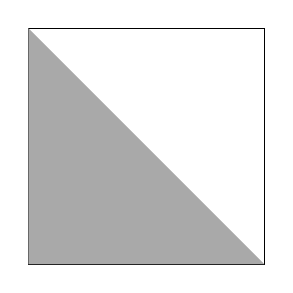
\begin{tikzpicture}
        \draw (0,0) rectangle (3,3);
        \fill[gray!90, opacity=0.75] (3, 0) -- (0, 0) -- (0, 3) -- cycle;
    \end{tikzpicture}
    \caption{General QUBO problem.}
    \label{fig:exstart}
\end{figure}

Once partitioned by the splitting operation, the result is what is presented in Figure \ref{fig:exsplit}, where of the four subproblems, only three require a solution to be aggregated.

\begin{figure}[H]
    \centering
    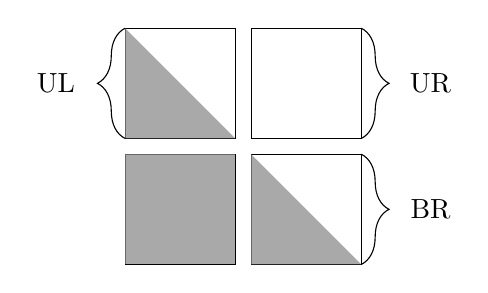
\begin{tikzpicture}
        \draw (0,0) rectangle (1.4,1.4);
        \draw (1.6,1.6) rectangle (3,3);
        \draw (0,1.6) rectangle (1.4,3);
        \draw (1.6,0) rectangle (3,1.4);
        \fill[gray!90, opacity=0.75] (0,0) -- (0,1.4) -- (1.4,1.4) -- (1.4,0);
        \fill[gray!90, opacity=0.75] (0,1.6) -- (0,3) -- (1.4,1.6) -- cycle;
        \fill[gray!90, opacity=0.75] (1.6,0) -- (3,0) -- (1.6,1.4) -- cycle;

        \draw[decorate,decoration={brace,amplitude=10pt}] (0,1.6) -- (0,3) node [black,midway,xshift=-25pt] {$\operatorname{UL}$};
        \draw[decorate,decoration={brace,amplitude=10pt,mirror}] (3,1.6) -- (3,3) node [black,midway,xshift=25pt] {$\operatorname{UR}$};
        \draw[decorate,decoration={brace,amplitude=10pt,mirror}] (3,0) -- (3,1.4) node [black,midway,xshift=25pt] {$\operatorname{BR}$};
    \end{tikzpicture}
    \caption{One step split.}
    \label{fig:exsplit}
\end{figure}

For each step of the recursive partition, three new problems are generated, which in turn can be further partitioned.

So, to handle a problem with $2^a$ variables by sending subproblems of size $2^b$ to the QPU, where $a \geq b$, means transmitting a total of $3^{a-b}$ subproblems to \texttt{QPUSampler}, where 3 is the number of subproblems generated by a single execution of the split step and $(a-b)$ is the number of recursive calls of \texttt{QSplitSampler}.

This calculation considers only the number of subproblems sent to the QPU by the splitting procedure. 
Conflict resolution also generates new subproblems, but their number grows linearly with the recursive calls of \texttt{QSplitSampler}. For this reason, its contribution may be disregarded as the growth in the number of subproblems is dominated by the base-3 exponentiation.

Thus, for a problem with $128$ variables ($2^7$) and a \emph{cut dim} of $2$, the number of subproblems transmitted is at least: $3^{7-1}=3^6=729$.

Although \texttt{QSplitSampler} allows for handling problems larger than the QPU limits (Section \ref{sec:qpu-res}), the proposed methodology is insufficient for solving problems of the size discussed in Section \ref{sec:qsvm-res}. 
The version of SVM used generates a problem with $32,768$ ($2^{15}$) variables, calculated according to Equation \eqref{eq:nodesnum}. 
Even assuming a \emph{cut dim} of $64$ ($2^6$), the number of problems to be sent to the QPU would be at least $3^{15-6}=3^9=19,683$.


\part{Discussion and Conclusion}

\chapter{Conclusion}

The research presented in this thesis has allowed for an in-depth exploration of:
\begin{enumerate}
    \item The effectiveness of adiabatic quantum computing when applied to natural language processing tasks;
    \item The study of the topological and architectural limitations of the current generation of quantum processing units (QPU);
    \item The development of hybrid solvers as alternatives to those proposed by D-Wave.
\end{enumerate}

\paragraph{Quantum Support Vector Machine} The study of machine learning models based on quantum technologies is a relatively new topic in the research landscape. 
Despite this, the potential to exploit quantum phenomena has piqued the interest of some researchers, who hope to achieve either performance or representational advantages.

Among the works on quantum machine learning using quantum annealing, we can cite those by Vladislav Golyanik and his research group 4DQV\footnote{\url{https://4dqv.mpi-inf.mpg.de/}}, whose research focuses on the field of computer vision\cite{qcv1}\cite{qcv2}.

In natural language processing, there are no significant contributions aimed at integrating quantum annealing and language models. 
The experiments conducted as part of this research demonstrate that quantum computing can provide tangible benefits compared to traditional optimization methods, warranting further investigation. 
Additionally, it becomes clear that the trade-off between convergence speed and solution quality remains a variable to be assessed on a case-by-case basis. 
However, quantum-based models add to the range of available options.

In scenarios where computational resources are limited, quantum annealing processes can enable the development of useful models on personal computers and embedded systems. 
The solutions generated by quantum machines prove to be good approximations when compared to state-of-the-art models. 
Furthermore, given the reduction in model complexity, quantum machine learning techniques offer:
\begin{itemize}
    \item Improved interpretability of results, a significant factor in certain application contexts such as the medical field;
    \item Lower resource consumption, facilitating faster prototyping of new solutions.
\end{itemize}

\paragraph{QPU Analysis} The analysis of the QPU revealed that the computational resources required by the minor embedding algorithm do not allow problems with more than 128 logical qubits to be solved directly using the QPU. 
Beyond this empirical limit, the current Pegasus architecture lacks sufficient physical qubits and adequate interconnections between qubits to express the problems.

These limitations could be partially addressed with the introduction of new QPU topologies. 
For instance, Zephyr proposes a greater number of qubits and a graph with a generally higher degree.

However, even though newer QPUs might allow for the handling of increasingly large problems, the available resources are unlikely to be sufficiently extensive to meet the requirements for tackling real-world problem sizes. 

Even with the potential development of increasingly efficient algorithms for minor embedding and topological solutions that facilitate easier problem mapping onto QPUs, it is unlikely that the current trajectory of quantum annealing technologies will evolve without using hybrid paradigms. 
This makes the development of freely accessible solvers, both specialized for specific tasks and general purposes, a central necessity.

\paragraph{Homebrewing a Hybrid Solver} The hybrid solver proposed and developed during this thesis, \texttt{QSplitSampler}, has as its primary goal the extensive use of available quantum resources, seeking to rebalance the workload between the CPU and QPU.
Which in D-Wave's proposal seems to be heavily skewed towards CPU-intensive use.

The approach used by \texttt{QSplitSampler} allows application in various settings, far beyond what is possible with QML. 
This is due to the fact that the algorithm is based on the structure of the QUBO problem.
The main advantage of working with general problems such as those described by QUBO models is that the proposed procedure becomes easily reusable and adaptable across different contexts, beyond SVM optimization.

Currently, there are no guarantees regarding the practical utility of quantum computing in machine learning. 
Some studies focus specifically on verifying whether the procedures currently in use can be simulated efficiently on classical computers. 
Among these, we can mention the work of Marco Cerezo\cite{qcnn}, in which the paradigm of quantum convolutional neural networks, widely adopted in the literature, was shown not to exploit quantum phenomena appropriately, making the architecture classically simulatable.

The development of general-purpose solvers thus represents a more ``cautious'' path forward. 
Even if it were demonstrated that quantum computing cannot be effectively leveraged for machine learning tasks, solving QUBO problems remains an NP-complete challenge. 
Consequently, having a method to solve NP-complete problems quickly is still of significant research interest, encouraging an approach that remains agnostic to the specific application context.

\texttt{QSplitSampler} proposes an alternative solving method to those found in the literature, which include:
\begin{itemize}
    \item Iterative methods for dividing variables into subproblems as in Tameem Albash et al.\cite{subqubo2};
    \item Polyphase strategies to fix an increasing number of variable values, Dennis Willsch et al.\cite{subqubo1}.
\end{itemize}

\texttt{QSplitSampler} recursively partitions the QUBO problem, relying on algebraic properties, to maximize QPU usage. 
While this approach is reasonable, there is no guarantee increasing the use of the QPU will lead to better solutions.

The conducted tests suggest that purely algebraic decomposition may not be an optimal strategy for converging toward the global optimum. 
In Chapter \ref{sec:future}, some experimental approaches that could be explored to improve the performance of \texttt{QSplitSampler} will be discussed.

\chapter{Future works}\label{sec:future}

Understanding the limitations of current QPUs and the pre-processing procedures associated with their use is essential to ensure their informed use. Recognising strengths and weaknesses enables a more conscious assessment of when and how to deploy quantum resources for a given problem.

Although the QPU topology may pose a constraint in developing efficient solutions, this is a structural limitation that cannot be circumvented. The development of new QPUs is currently being explored by D-Wave, where it is reasonable to assume that technical experts accustomed to working closely with hardware are heavily involved.

From a computer science perspective, it is possible to ``limit'' ourselves to understand the available resources and leverage current tools most effectively. For this reason, the primary research directions that merit further investigation, beyond the work conducted in this thesis, include the following:

\begin{itemize}
    \item Reduction of the SVM problem into QUBO form, resulting in optimisation to classify examples from sentiment analysis (Section \ref{sec:qnlp});
    \item Developing alternative hybrid solvers (Section \ref{sec:bettersolver}).
\end{itemize}

\section{Quantum Natural Language Processing}\label{sec:qnlp}

Utilizing quantum annealing processes to optimize the support vector machine model has proven to be a successful strategy compared to state-of-the-art classical optimizers. Although the contribution of the QPU is marginal according to the data gathered in Section \ref{sec:qpuusage}, D-Wave's proprietary technology prevents further investigation. This is a significant limitation, suggesting that future research should not focus on methods to accelerate the training of models using D-Wave's solvers.

Since Section \ref{sec:dataset-full} revealed that increasing the number of examples does not correspond to an improvement in performance, reducing the size of the input dataset could be a way further to reduce the training time of the quantum annealing-based model. This would lead to:
\begin{itemize}
    \item A reduction in training times;
    \item A model that is faster to create and transfer to the cloud infrastructure due to the smaller size.
\end{itemize}
It remains to be verified to what extent the dataset size can be reduced without degrading the model's performance.

The performance of the quantum model when compared to state-of-the-art Transformer models is a different matter. As discussed in Section \ref{sec:qsvm-performance}, the difference between the proposed solution and RoBERTa is substantial, making the quantum approach unsuitable for cases where the cost of inference errors outweighs the longer training times required by the model.

The main directions for improving the proposed model include:
\begin{itemize}
    \item Investigating model parameterization;
    \item Using different textual embeddings;
    \item Leveraging SVMs in deep learning contexts;
    \item Exploring alternative models.
\end{itemize}

\paragraph{Problem Parameterization} As with the dataset size used in training, the model's parameterization was not deeply explored during the development of this thesis.

The parameter $C$ (Section \ref{sec:soft}) was initially set to $255$ because:
\begin{itemize}
    \item The performance obtained was significantly better than random guessing;
    \item The focus of the thesis was on studying quantum solvers.
\end{itemize}
No other parameter combinations were tested, but finding an optimal value for $C$ could improve the model’s performance by a few percentage points.

It should be noted, however, that even with improved performance, different parameterizations are unlikely to surpass the results achieved by RoBERTa, given the limitations of the SVM model when applied to linguistic tasks.

\paragraph{Exploring Better Embeddings} Section \ref{sec:embeddingused} defined the procedure used to generate textual embeddings.

To fully understand the limitations of the SVM model, it is necessary to estimate the contribution of the embedding to the classification task. Comparing model performance using different embeddings, while also considering the time required to produce them, may provide a valuable avenue for further investigation.

Possible alternative embeddings could include:
\begin{itemize}
    \item Embeddings derived from more task-specific models, specifically developed for sentiment analysis;
    \item Embeddings generated by aggregating the information on the word level, instead of using the current procedure that directly generates an embedding for the entire sentence;
    \item Manually constructed embeddings based on descriptive features obtained from an exploratory dataset analysis.
\end{itemize}

\paragraph{Multiple SVM Approaches} Instead of using a single SVM for classification, strategies involving an ensemble of models could be employed. If the number of trained SVMs is kept sufficiently low, training multiple models would still be significantly faster than the time required for Transformers, potentially achieving comparable performance.

The main methodologies that could be explored include:
\begin{itemize}
    \item Implementing an ensemble learning algorithm\cite{adaboost}, which unlike the experiments conducted, provides each model in the ensemble with a different partition of the dataset;
    \item Deep learning approaches based on SVMs, such as those proposed by Jingyuan Wang et al. in \cite{deepsvm}.
\end{itemize}

\paragraph{Alternative Models} All previous proposals are based on improving the SVM model and finding methods to enhance its performance or expressive capacity.

Although the dual formulation of SVMs makes quantum annealing a natural fit, it is possible to study the reduction of alternative machine learning and deep learning models into quadratic programming problems. The best way to close the gap between QSVM and RoBERTa may lie in adopting a new model. In this case, it would be necessary to evaluate:
\begin{itemize}
    \item The cost of reformulating the problem;
    \item The complexity of the resulting model, as different models may be too complex for current hybrid solvers.
\end{itemize}

\section{Improving Current Quantum Solvers}\label{sec:bettersolver}

The second area where this thesis could be further developed involves \texttt{QSplitSampler}, the open-source hybrid solver developed as an alternative to D-Wave's offerings.

The proposed algorithm has room for improvement in both its use of quantum resources and its execution of local code.

\paragraph{Classical Component} Although the current code is reasonably efficient and does not represent the main bottleneck during execution, it could still be optimized.

\subparagraph{Vectorization of Calculations} Currently, calculations are performed as outlined in Section \ref{sec:qsplitimplementation}. By leveraging vectorization techniques such as SIMD (Single Instruction Multiple Data), repetitive operations can be handled more efficiently using modern CPU architectures.

\subparagraph{Parallelizing the Procedure} Since the splitting process generates subproblems that can be handled independently, it is possible to parallelize the recursive subdivision, awaiting results for the aggregation phase. However, it should be noted that part of the performance gains from parallelization may be offset by the quantum component. Once the problems are sent to D-Wave's cloud infrastructure, they are queued and solved one at a time. This behaviour limits the potential of parallel programming. It may still be worth further investigation since QPU solutions appear fast enough to potentially reduce average wait times if D-Wave is provided with multiple problems to solve in sequence.

\paragraph{Quantum Component} While it is possible to start ``from scratch'' to develop new open-source solvers capable of leveraging different properties of the problems being tackled, it could be interesting from a research perspective to explore the limits of \texttt{QSplitSampler} by improving some ``critical'' aspects that emerged during its development and use.

\subparagraph{Diversifying Partitioning Strategies} As an alternative to the current approach, QUBO problems could be divided based on the structure of the problem. For example, in cases where a significant portion of the problem consists only of zero coefficients, the subproblem size could be increased, as the resulting graph would remain small enough to compute the minor embedding and execute on the currently available QPUs.

\subparagraph{Different Allocation Between CPU and QPU} Currently, all subproblems generated by \texttt{QSplitSampler} are sent to the QPU. By reducing the quantum contribution in the solution search, it could be considered a quick analysis of problems to determine whether to send them to the QPU or solve them using the CPU. As with the development of an alternative partitioning strategy, the main challenge with this approach would be finding an efficient heuristic to evaluate the problems without negatively impacting the overall performance of the algorithm.

\subparagraph{Incorporating \texttt{QSplitSampler} into Hybrid Pipelines} Creating pipelines represents a special case of workload distribution between CPU and QPU. Even assuming \texttt{QSplitSampler} remains unchanged, the solutions it produces could be used as starting points for local search techniques. This approach was originally used by D-Wave in the now-deprecated \texttt{QBSolv}\footnote{\url{https://github.com/dwavesystems/qbsolv}} library. Alternating quantum search processes with classical searches in the state space could be a compromise capable of accelerating the search without negatively impacting solution quality.


\printbibliography

\end{document}